\documentclass[times, twoside]{zHenriquesLab-StyleBioRxiv}
\usepackage{bm}
\usepackage{booktabs}
\usepackage{graphicx}

\leadauthor{Ikari}

\begin{document}

\title{Route Correction and Variance Decomposition for Aerobic Decoupling: A 13K-Workout Study of Durability Dimensionality}
\shorttitle{Route Correction for Aerobic Decoupling}

\author[1,\Letter]{Hisashi Ikari}

\affil[1]{Independent Researcher}

\maketitle



%TC:break Abstract
\begin{abstract}
Millions of athletes use the speed-based Decoupling Index (DI) displayed by GPS-watch platforms such as TrainingPeaks and Strava, yet its sensitivity to route geometry has never been quantified. This study analysed $N = 13{,}750$ real-world workouts from $K = 675$ users to examine whether route terrain---rather than physiological cardiac drift---dominates speed-based DI, and to test the empirical dimensionality of the four-construct durability framework proposed by Meixner et al.\ (2025). Three speed-based indices were defined: DI (durability), the Fading Index (FI; fatigability), and the Resilience Index (RI; resilience). A controlled simulation ($N = 5{,}000$ synthetic workouts with zero cardiac drift) showed that route geometry alone produces DI values ranging from 0.70 to 1.40 (cross-validated $R^2 = 0.80$). In real data, route features predicted DI with $R^2 = 0.49$; after Gradient-Adjusted Cardiac Drift (GACD) regression, this predictability was eliminated ($R^2 \approx 0.02$). Notably, 42\% of routes were front-climb profiles that mechanically produce DI $< 1.0$ even with zero cardiac drift, suggesting widespread misinterpretation of this metric on hilly terrain. PCA on person-level medians retained one factor; the second eigenvalue (1.005) fell marginally below the parallel-analysis threshold (1.031), providing fragile support for a two-construct organisation in which DI and FI are redundant ($r = -0.60$) while RI appears independent but unreliable (ICC $= 0.10$). Variance decomposition revealed that day-to-day Occasion variance dominates all metrics (56--84\%), necessitating multi-session aggregation: gradient sensitivity from the GACD regression reached adequate reliability (Spearman--Brown $\geq 0.80$) at $k \geq 5$ sessions. Sport-specific analysis confirmed that the Occasion-dominant pattern holds for cycling (Occasion 50--78\% across the three GACD-derived metrics); the running subsample was too small for stable estimation. These findings demonstrate that speed-based DI is heavily contaminated by route geometry and that gradient-adjusted, multi-session profiling provides a more reliable individual signal for longitudinal durability monitoring.
\end{abstract}
%TC:break main

\begin{keywords}
aerobic decoupling | durability | cardiac drift | heart rate | gradient sensitivity | measurement artifact | field testing
\end{keywords}

\begin{corrauthor}
hisashi\at ikari.io
\end{corrauthor}

% ============================================================
\section*{Introduction}

Aerobic decoupling---the progressive rise in heart rate (HR) relative to pace or power during prolonged exercise---has been widely adopted as a field-based indicator of endurance fitness \cite{coyle2001, friel2009}. Platforms such as TrainingPeaks and Strava present the Decoupling Index (DI) to millions of athletes, applying Friel's $<5\%$ threshold to indicate adequate aerobic base. This threshold has never been empirically validated in a peer-reviewed study. The most closely related large-scale study is Smyth et al.\ \cite{smyth2022}, who characterised internal-to-external workload decoupling in 82,303 marathon runners and demonstrated that both decoupling magnitude and onset are associated with performance. Their work establishes the ecological validity of field-based decoupling measurement at scale, but did not examine the route-geometry artifact, the dimensional structure of multiple decoupling indices, or the variance attributable to person, route, and occasion---the gaps addressed here.

On variable terrain, speed---determined primarily by gradient---is an imperfect proxy for external workload, introducing a route-geometry component into speed-based DI. What has not been established is (a)~the magnitude of this component, (b)~whether it dominates physiological signal in real-world data, and (c)~what meaningful signal remains once it is corrected.

Meixner et al.\ \cite{meixner2025} proposed four conceptual constructs for endurance durability: durability, fatigability, repeatability, and resilience. The accompanying commentaries---Colosio et al.\ \cite{colosio2025} on physiological distinctions, Faude et al.\ \cite{faude2025} on methodological gaps, Lucernoni et al.\ \cite{lucernoni2025} on reconceptualising resilience, and the authors' rebuttal \cite{meixner2025last}---reveal an active debate over whether these four constructs are empirically separable, with no consensus yet reached. Separately, Jones \cite{jones2024} proposed physiological resilience as a fourth independent determinant of endurance performance, providing theoretical grounding for the resilience construct. All discussions have remained at the conceptual level. To bridge theory and large-scale field data, this study introduces three author-defined operationalizations of Meixner et al.'s constructs: the Decoupling Index (DI; operationalizing durability), the Fading Index (FI; fatigability), and the Resilience Index (RI; resilience). The fourth construct (repeatability) was not operationalized in this study due to the absence of repeated-bout protocols in the FitRec dataset. These indices are not defined in Meixner et al.\ \cite{meixner2025}; they are original operationalizations designed to map the theoretical constructs to measurable GPS and HR field data. One likely reason no prior large-scale study exists is a disciplinary gap: Meixner et al.'s framework defines DI as $\text{HR}/\text{Power}$, while the FitRec dataset \cite{ni2019}---published in the recommender-systems community---contains HR and GPS but no power data. Yet the majority of real-world users compute $\text{HR}/\text{Speed}$ via consumer GPS watches. This study does not challenge the theoretical constructs themselves; rather, it examines the empirical structure that emerges when those constructs are operationalized with the speed-based metrics that millions of users actually employ, a necessity for field-based durability research \cite{hunter2025}. While Friel (2009) \cite{friel2009} proposed a 5\% DI threshold for physiological decoupling, the present results suggest that on variable terrain, this index is heavily contaminated by route-geometry artifacts, necessitating a more robust gradient-adjusted approach. This distinction---between theoretical construct validity and field-level operationalization---is the central concern of the present work.

The reliability of field-based HR metrics has long been a concern \cite{hopkins2000, halson2014}. The IOC consensus \cite{bourdon2017} emphasized the external-load/internal-response distinction, but no study has quantified the variance attributable to person, route, and occasion in HR-response metrics.

\subsection*{Research Questions}

All analyses use speed-based DI ($\text{HR}/\text{Speed}$), not power-based DI ($\text{HR}/\text{Power}$), because no power data are available in FitRec. Results apply to the majority of real-world users who compute DI via consumer GPS watches. It should be noted that HR/Speed is a pragmatic but theoretically limited proxy for cardiac efficiency in cycling---where speed is determined by power output, gradient, aerodynamic drag, and rolling resistance---and a stronger proxy in running, where speed is more directly related to metabolic cost on flat terrain. The implications of this distinction for the cycling-dominated dataset (61.8\%) are addressed in the Discussion.

\textbf{CRQ1: What is the empirically supported dimensionality of the durability framework under speed-based DI?}
\begin{itemize}
  \item[\textbf{H1}] DI and FI collapse onto a single construct, tentatively supporting a two-construct organisation.
  \item[\textbf{H2}] All durability dimension ICCs fall below 0.50, indicating insufficient reliability for four independent dimensions.
  \item[\textbf{H3}] DI route predictability vanishes after gradient correction (GACD), confirming that the route-geometry component can be effectively removed.
\end{itemize}

\textbf{CRQ2: To what extent do stable individual physiology, route properties, and transient daily state each account for the variance in HR-response metrics?}
\begin{itemize}
  \item[\textbf{H4}] Transient daily state (Occasion) accounts for $>50\%$ of variance, necessitating multi-session aggregation for reliable measurement.
\end{itemize}

Three exploratory hypotheses were also examined:
\begin{itemize}
  \item[\textbf{E1}] Temporal placement of descent affects cardiac drift.
  \item[\textbf{E2}] A more stable HR parameter than DI exists.
  \item[\textbf{E3}] ICC $\ll$ split-half reliability (rank-order stability $>$ absolute consistency).
\end{itemize}

\subsection*{Contributions}

\textbf{C1}~Fragile support for a two-construct organisation (PCA retained one factor; PC2 = 1.005, marginally below threshold 1.031; the small margin of 0.026 eigenvalue units warrants caution), with quantification of the route-geometry artifact ($R^2 = 0.80$; 2-fold range) and demonstration that naive power estimation overcorrects. \textbf{C2}~A large-scale variance decomposition (Person/Route/Occasion) for HR-response metrics: the same person on the same route shows 26--54\% day-to-day variation, indicating that the four-construct operationalization requires multi-session aggregation to be reliably measured. \textbf{C3}~A between-person association between descent placement and cardiac drift, with modest within-person support. \textbf{C4}~Convergence analysis showing that gradient sensitivity requires $\geq 5$ sessions for adequate reliability.


% ============================================================
\section*{Methods}

\subsection*{Data and Filtering}

The FitRec dataset \cite{ni2019} was used, comprising 253,020 GPS-tracked workouts from Endomondo. Each workout record $j$ contains irregularly time-stamped arrays of heart rate ($\mathit{HR}_{j,i}$, optical wrist sensor, $\mathrm{bpm}$), speed ($v_{j,i}$, GPS-derived, $\mathrm{km{\cdot}h^{-1}}$ in the raw data), altitude ($a_{j,i}$, barometric or GPS-derived, $\mathrm{m}$), and geographic coordinates, where $i = 1, \ldots, N_j$ indexes the data points. Where the recorded speed array was missing or shorter than 10 points, speed was derived from GPS coordinates via the Haversine formula (values exceeding $150\,\mathrm{km{\cdot}h^{-1}}$ were excluded as outliers). The gender variable indicates 94.6\% male, 4.8\% female, 1.2\% unknown; age, body mass, and training history are unavailable. Sensor make and firmware version are not recorded.

A four-step inclusion pipeline was applied: (1)~HR, altitude, and speed arrays each required $N_j \geq 30$ finite data points (a minimum for stable within-half mean estimation with $\geq 15$ points per half); missing values were linearly interpolated between flanking valid points; (2)~total duration $T_j = t_{N_j} - t_1 > 90\,\mathrm{min}$, ensuring sufficient exercise duration for cardiac drift to manifest \cite{coyle2001}; (3)~altitude range $\Delta a_j = \max_i(a_i) - \min_i(a_i) > 200\,\mathrm{m}$, a conservative threshold for ensuring sufficient gradient variation to confound the speed-based DI (approximately the lower quartile of the retained dataset; median $= 349\,\mathrm{m}$). To address sensor-induced barometric drift, the start-to-end altitude deviation was required to satisfy $|\Delta a_{\text{drift}}| = |a_{N_j} - a_1| < 50\,\mathrm{m}$ for routes suspected to be loops ($> 80\%$ overlap); (4)~each temporal half (H1: $i \leq \lfloor N_j/2 \rfloor$; H2: $i > \lfloor N_j/2 \rfloor$) required $> 5$ points with $v_i > 0.5\,\mathrm{km{\cdot}h^{-1}}$ (i.e., $\geq 6$ per half), where $0.5\,\mathrm{km{\cdot}h^{-1}}$ excludes stationary GPS noise while preserving low-speed segments on steep climbs. When speed was entirely unavailable, a heart-rate-only DI ($= \bar{\text{HR}}_{\text{H2}} / \bar{\text{HR}}_{\text{H1}}$) was computed as a fallback; FI and RI required speed.

This yielded $N = 13{,}750$ workouts from $K = 675$ users for Study~1 (cycling 61.8\%, running 16.9\%, mountain biking 16.7\%, other 4.6\%; median duration $181\,\mathrm{min}$). Studies~2--3 required $\geq 5$ repeated workouts per user, yielding a high-engagement subset of $N = 2{,}343$ workouts from $K = 314$ users (cycling 83.9\%, running 7.6\%, mountain biking 5.8\%, other 2.7\%; median duration $208\,\mathrm{min}$ [IQR 152--298]).

\subsection*{Metric Definitions}

Speed in the raw data is recorded in $\mathrm{km{\cdot}h^{-1}}$ (metrics 1--3). For the within-workout regression (metrics 4--6), speed was converted to $\mathrm{m{\cdot}s^{-1}}$ ($\div 3.6$); the gradient computation uses speed in $\mathrm{m{\cdot}s^{-1}}$ and timestamps in seconds.

\textbf{(1) Decoupling Index (DI).} Let $\mathcal{S}_h = \{i \in \text{H}_h : v_i > 0.5\,\mathrm{km{\cdot}h^{-1}}\}$ for $h \in \{1, 2\}$. The DI is:
\[
  \text{DI} = \frac{\bar{\text{HR}}_{\mathcal{S}_2} \,/\, \bar{v}_{\mathcal{S}_2}}{\bar{\text{HR}}_{\mathcal{S}_1} \,/\, \bar{v}_{\mathcal{S}_1}}
\]
where $\bar{\text{HR}}_{\mathcal{S}_h} = |\mathcal{S}_h|^{-1}\sum_{i \in \mathcal{S}_h} \text{HR}_i$ and analogously for $\bar{v}$. DI $> 1$ indicates cardiac drift.

\textbf{(2) Fading Index (FI).} For FI, point-to-point gradient was computed from the cumulative horizontal distance: $D_i = \sum_{l=1}^{i} v_l \cdot \Delta t_l / 3600 \times 1000\,\mathrm{(m)}$, with minimum horizontal step $0.1\,\mathrm{m}$, and $g_i = \text{clip}(100 \times \Delta a_i / \Delta D_i,\; -50,\; +50)\,\%$. The gradient range was partitioned into five bins $\mathcal{B}_b$: $[-50,-10)$, $[-10,-3)$, $[-3,3)$, $[3,10)$, $[10,50)\,\%$, following the conventional gradient classification used by commercial training platforms (flat: $< 3\%$; moderate: $3$--$10\%$; steep: $> 10\%$):
\[
  \text{FI}_b = \frac{\bar{v}_{\mathcal{S}_2 \cap \mathcal{B}_b}}{\bar{v}_{\mathcal{S}_1 \cap \mathcal{B}_b}}, \quad \text{FI} = \frac{1}{|\mathcal{B}^*|} \sum_{b \in \mathcal{B}^*} \text{FI}_b
\]
where $\mathcal{B}^* = \{b : |\mathcal{S}_1 \cap \mathcal{B}_b| > 3 \text{ and } |\mathcal{S}_2 \cap \mathcal{B}_b| > 3\}$. Of the $N = 13{,}742$ workouts with valid FI (Table~\ref{tab:descriptive}), 99.9\% had at least one gradient bin populated in both halves; FI was undefined for the remaining 8 workouts.

\textbf{(3) Resilience Index (RI).} The RI operationalizes the resilience construct proposed by Jones \cite{jones2024}, who identified physiological resilience as a fourth independent determinant of endurance performance. This operationalization is a preliminary proxy: Jones (2024) defines resilience in terms of preservation of physiological profiling variables (VO$_2$max, economy, critical power) under fatigue, whereas RI captures only speed maintenance between the first and last climb---a gap that future studies with laboratory-grade measurements could address. Three additional confounds are noted: (a)~the relative steepness of $C_1$ vs.\ $C_m$ is not controlled; (b)~temporal position of climbs within the workout is not normalised; (c)~RI values are not directly comparable across workouts with different numbers of climbs $m$. Altitude was smoothed by a trailing moving average (window $w = \max(1, \lfloor N/20 \rfloor)$, mode = ``valid''), yielding a smoothing window of approximately 5\% of the workout duration; this balances noise reduction against oversmoothing of true elevation changes. A climb was initiated when the smoothed altitude increased by $> 0.5\,\mathrm{m}$ from one point to the next, and terminated when this condition ceased; only climbs with cumulative vertical gain $> 50\,\mathrm{m}$ were retained. This threshold is an author-defined pragmatic choice informed by cycling industry convention (the FIETS climb index \cite{fiets}), not a peer-reviewed standard; sensitivity to this threshold was not formally assessed. Let $C_1, \ldots, C_m$ denote the retained climbs. If $m \geq 2$:
\[
  \text{RI} = \bar{v}_{C_m} / \bar{v}_{C_1}
\]
where $\bar{v}_{C_l} = |\{i \in C_l : v_i > 0.5\}|^{-1} \sum_{i \in C_l,\, v_i > 0.5} v_i$.
Workouts with $m < 2$ received no RI.

\textbf{(4--6) Within-workout regression.} For the regression-derived metrics, speed was in $\mathrm{m{\cdot}s^{-1}}$ and gradient was computed as:
\begin{align*}
  g_i &= \text{clip}\!\left(100 \times \frac{a_{i+1} - a_i}{d_i},\; -50,\; +50\right), \\
  d_i &= \max(v_i \cdot \Delta t_i,\; 0.1\,\mathrm{m}), \quad \Delta t_i = \max(t_{i+1} - t_i,\; 0.1\,\mathrm{s})
\end{align*}
Note that the minimum distance floor is $0.1\,\mathrm{m}$ (not $0.5\,\mathrm{m}$ as in FI), reflecting the finer resolution needed for regression. All variables were evaluated at midpoints: $\text{HR}^*_i = (\text{HR}_i + \text{HR}_{i+1})/2$, $v^*_i = (v_i + v_{i+1})/2$, $t^*_i = (t_i + t_{i+1})/2\,\mathrm{(min)}$. On the subset of valid indices ($|\mathcal{V}| \geq 20$ required), the OLS regression:
\begin{align}
  \mathit{HR}^*_i &= \beta_0 + \beta_{\text{grad}} \, g_i + \beta_{\text{speed}} \, v^*_i + \beta_{\text{time}} \, t^*_i + \varepsilon_i, \label{eq:gacd} \\
  \hat{\boldsymbol{\beta}} &= (\mathbf{X}^\top \mathbf{X})^{-1} \mathbf{X}^\top \mathbf{y} \nonumber
\end{align}
Linearity was confirmed via residual analysis, with homoscedasticity observed across the primary speed and gradient ranges. Importantly, $\beta_{\text{time}}$ captures the within-session rate of HR drift after controlling for gradient and speed; this should be distinguished from the between-session durability construct defined by Maunder et al.\ \cite{maunder2021}, which concerns shifts in the power--duration relationship after a fatiguing bout.

\subsection*{Sensitivity Analysis: Temporal Autocorrelation}

Point-level GPS data exhibit temporal autocorrelation, which violates the OLS assumption of independent errors. To quantify its impact, a sensitivity analysis was conducted on a random subsample of $N = 300$ workouts (median $n = 499$ data points per workout). For each workout, the GACD regression was re-run and the following diagnostics computed:

\textbf{Durbin--Watson (DW) statistics.} The DW statistic was computed as $DW = \sum_{t=2}^{n}(e_t - e_{t-1})^2 / \sum_{t=1}^{n} e_t^2$, where $e_t$ are OLS residuals. A value of 2.0 indicates no autocorrelation. The median DW was 0.355 (IQR: 0.245--0.501), and 100\% of workouts showed strong positive autocorrelation (DW $< 1.5$; Supplementary Figure~\ref{fig:dw}).

\textbf{Autocorrelation function (ACF).} The lag-1 autocorrelation of GACD residuals was high (median $\rho_1 = 0.803$, IQR: 0.735--0.862; Supplementary Figure~\ref{fig:acf}), with substantial autocorrelation persisting to lag 10+. Under an AR(1) approximation, the effective sample size is reduced by a median of 89\% ($n_{\text{eff}}/n = 0.109$).

\textbf{Newey--West HAC standard errors.} To assess the impact on inference, Newey--West heteroskedasticity- and autocorrelation-consistent (HAC) standard errors were computed with a Bartlett kernel and bandwidth $L = \lfloor 4(n/100)^{2/9} \rfloor$. The HAC standard errors were approximately 2$\times$ larger than OLS standard errors across all coefficients (median SE ratio: $\beta_{\text{gradient}}$: 2.03; $\beta_{\text{time}}$: 2.12; $\beta_{\text{speed}}$: 2.06). A caveat applies: under strong persistence ($\rho_1 \approx 0.80$), standard Newey--West HAC can itself be unreliable, potentially underestimating the true SE inflation \cite{lazarus2018}; the reported $\sim$2$\times$ ratio should therefore be considered a lower bound. Crucially, OLS point estimates ($\hat{\boldsymbol{\beta}}$) remain unbiased under autocorrelation; only the standard errors are underestimated. The primary quantity of interest for individual profiling is the point estimate of the regression coefficients rather than inference on individual session slopes, and OLS was retained for its computational efficiency in a high-throughput pipeline. Per-workout $R^2$ values should be interpreted as upper-bound estimates of model fit.
where $\mathbf{X} \in \mathbb{R}^{|\mathcal{V}| \times 4}$ (intercept, $g$, $v^*$, $t^*$) yielded: (4)~GACD ($\hat{\beta}_{\text{time}}$, $\mathrm{bpm{\cdot}min^{-1}}$); (5)~Gradient sensitivity ($\hat{\beta}_{\text{grad}}$, $\mathrm{bpm{\cdot}\%^{-1}}$); (6)~Speed sensitivity ($\hat{\beta}_{\text{speed}}$, $\mathrm{bpm{\cdot}(m{\cdot}s^{-1})^{-1}}$). Per-workout $R^2 = 1 - \|\mathbf{y} - \mathbf{X}\hat{\boldsymbol{\beta}}\|^2 / \|\mathbf{y} - \bar{y}\mathbf{1}\|^2$. Point-level gradients were clipped to $\pm 50\%$, as values beyond this range exceed the steepest rideable/runnable terrain and indicate sensor artifacts. Although gradient ($g_i$) and speed ($v^*_i$) exhibit collinearity in field environments, multicollinearity was minimal (median VIF: gradient 2.01, speed 2.09, time 1.07), with 99.8\% of sessions falling below the VIF $< 10$ threshold (92.4\% below 5) \cite{hair2010}.

\subsection*{Estimated Power Experiment}

DI was recomputed with the denominator replaced by estimated metabolic power $P_i = v_i \cdot C_w(g_i)\,\mathrm{(W{\cdot}kg^{-1})}$, where $C_w(g)$ is the Minetti \cite{minetti2002} gradient cost of walking transport ($\mathrm{J{\cdot}kg^{-1}{\cdot}m^{-1}}$), computed from the published 5th-order polynomial (Eq.~2 of Minetti et al., 2002):
\[
  C_w(i) = 280.5\,i^5 - 58.7\,i^4 - 76.8\,i^3 + 51.9\,i^2 + 19.6\,i + 2.5
\]
where $i$ is gradient as a fraction (e.g., $i = 0.10$ for 10\%), valid for $i \in [-0.45, +0.45]$. Values were floored at $0.1\,\mathrm{J{\cdot}kg^{-1}{\cdot}m^{-1}}$ to prevent near-zero denominators on moderate descents:
\[
  \text{DI}_{\text{EstP}} = \frac{\bar{\text{HR}}_{\mathcal{S}_2} \,/\, \bar{P}_{\mathcal{S}_2}}{\bar{\text{HR}}_{\mathcal{S}_1} \,/\, \bar{P}_{\mathcal{S}_1}}
\]
The metabolic cost of transport was estimated using the 5th-order polynomial published by Minetti et al. (2002) \cite{minetti2002}. To ensure robust estimation, extreme outliers were removed using 1st and 99th percentile trimming \cite{wilcox2012}, resulting in a final sample of $N = 13{,}080$ for the power-estimation experiments. Prolonged exercise was defined as $T > 90\,\mathrm{min}$, consistent with the manifesting period for cardiovascular drift \cite{coyle2001, acsm2018}. Note that the Minetti cost function was originally derived for human walking and running; its application to a dataset dominated by cycling (61.8\%) introduces an inherent bioenergetic mismatch (see Discussion).

\subsection*{Study~1: Construct Validity --- H1 (DI--FI redundancy), H2 (ICC $< 0.50$)}

To test whether the proposed four dimensions are empirically distinct (H1) and individually reliable (H2), person-level medians of DI, FI, and RI were computed for each user with $\geq 5$ workouts ($N = 13{,}750$; for RI, $N = 10,032$). Median-based aggregation was selected due to high Kurtosis (e.g., 590 for FI) indicating extreme outliers and heavy-tailed distributions. Pairwise Pearson correlations were estimated via nonparametric bootstrap ($B = 2{,}000$; users resampled with replacement; 95\% CI from 2.5th and 97.5th percentiles). 
If H1 holds, DI and FI should show a strong negative correlation (FI $< 1$ when DI $> 1$) and PCA should retain only one factor.

PCA was performed on column-standardised person-level medians ($z_{ij} = (x_{ij} - \bar{x}_j) / s_j$) for users with valid values on all three metrics. Factor retention was determined by parallel analysis \cite{horn1965}: observed eigenvalues were compared to the 95th percentile of eigenvalues from $B = 1{,}000$ column-wise random permutations of standard normal data of the same dimensions. ICC(1,1) was selected as the reliability metric because workouts are unique, non-overlapping samples per user and cannot be treated as crossed or fixed factors; thus, 2-way models (ICC(2,1), ICC(3,1)) are inappropriate for this dataset. ICC(1,1) was computed for each metric on users with $\geq 5$ workouts (see Study~3); H2 predicts all ICCs $< 0.50$.

\textbf{Robustness check.} To ensure that the findings were not artifacts of specific inclusion thresholds, a sensitivity analysis was performed by varying $T_{\text{min}}$ from 60 to 120\,min and $\Delta a$ from 100 to 300\,m. Across all 25 combinations, the DI--FI correlation remained remarkably stable ($\bar{r} = -0.60$, SD $= 0.02$, range $[-0.63, -0.57]$), confirming that the observed redundancy is a robust phenomenon independent of specific filtering choices.

\subsection*{Study~2: Route-Geometry Correction --- H3 (gradient correction), E1 (descent placement)}

\textbf{Route prediction.} Let $\mathbf{x}_j \in \mathbb{R}^{13}$ denote 13 route features (total ascent/descent, altitude range, max/min altitude, gradient mean/std, climb/descent/flat fractions, ascent-front and descent-front ratios, duration). Within each cross-validation fold $f$, features were $z$-standardised using training-fold statistics only ($\mu^{(f)}_p$, $\sigma^{(f)}_p$ computed on $\text{train}_f$; applied to both $\text{train}_f$ and $\text{test}_f$), and RidgeCV regression (selecting $\alpha \in \{0.01, 0.1, 1.0, 10, 100\}$ via internal leave-one-out CV) was fitted:
\[
  \hat{\boldsymbol{\beta}}_{\text{ridge}} = (\mathbf{X}^\top \mathbf{X} + \alpha \mathbf{I})^{-1} \mathbf{X}^\top \mathbf{y}, \quad \alpha^* = \arg\min_{\alpha} \text{LOO-CV}(\alpha)
\]
and gradient boosted trees (100 trees, max depth 3) were fitted. Generalisation was assessed by group $k$-fold cross-validated $R^2$ ($k = \min(5, K_{\text{valid}})$; all workouts of each user in the same fold):
\[
  R^2_{\text{CV}} = 1 - \frac{\sum_{f=1}^{k} \sum_{j \in \text{test}_f} (y_j - \hat{y}_j^{(f)})^2}{\sum_{f=1}^{k} \sum_{j \in \text{test}_f} (y_j - \bar{y})^2}
\]
The hilly subset was restricted to $\Delta a_j > 400$~m. For GACD, the target was the within-person deviation $\tilde{y}_{kj} = y_{kj} - \bar{y}_{k\cdot}$ (users with $\geq 3$ workouts), isolating route effects from person-level means.

\textbf{Empirically-parameterised controlled experiment.} $N = 5{,}000$ synthetic workouts ($N_{\text{pts}} = 60$, split at 30) were generated with cardiac drift set exactly to zero. All distributional parameters were derived from the FitRec dataset. Three route types were sampled with empirical proportions (classified by ascent-front ratio from \texttt{abc\_metrics.csv}, $N = 2{,}343$):
\begin{itemize}
  \item Front-climb (asc\_front $> 0.6$; 42.2\%): $g_{\text{H1}} \sim \mathcal{N}(+1.0, 1.84^2)$,\; $g_{\text{H2}} \sim \mathcal{N}(-1.0, 1.84^2)$
  \item Back-climb (asc\_front $< 0.4$; 10.2\%): reversed
  \item Symmetric ($0.4 \leq$ asc\_front $\leq 0.6$; 47.6\%): $g \sim \mathcal{N}(0, 1.84^2)$ throughout
\end{itemize}
The gradient asymmetry ($\pm 1.0\%$) was derived from the ascent-front distribution (front-climb mean $\approx 0.69$), and the point-level gradient standard deviation ($1.84\%$) was chosen to produce realistic gradient profiles (the actual per-workout gradient standard deviation in the dataset is larger, mean $= 4.96\%$, reflecting the wider range of terrain in hilly workouts; the simulation uses a smaller value appropriate for moderate terrain). Per-workout physiological parameters were sampled from FitRec-derived distributions: $\text{HR}_0 \sim U(107, 159.5)$ (P5--P95 of \texttt{avg\_hr} in the full dataset, $N = 13,750$), $\gamma_{\text{HR}} \sim \max(0.1,\; \mathcal{N}(1.91, 1.48^2))$~bpm/\% (from \texttt{gacd\_gradient\_coef}), $v_0 \sim \max(1.0,\; \mathcal{N}(1.91, 0.44^2))$~m/s, $\gamma_v \sim \max(0.01,\; \mathcal{N}(0.27, 0.15^2))$~(m/s)/\% (derived from Minetti \cite{minetti2002} cost function gradients). The data-generating process was:
\[
  \text{HR}_i = \text{HR}_0 + \gamma_{\text{HR}} \cdot g_i + \epsilon^{\text{HR}}_i, \quad \epsilon^{\text{HR}}_i \sim \mathcal{N}(0, 3^2)
\]
\[
  v_i = \max\!\left(0.5,\; v_0 - \gamma_v \cdot g_i + \epsilon^v_i\right), \quad \epsilon^v_i \sim \mathcal{N}(0, 0.3^2)
\]
No time-dependent term was included; any non-unity DI arises purely from gradient asymmetry between halves. The only experimentally controlled variable is cardiac drift $= 0$; all other parameters reflect empirical distributions from the dataset under study.

\textbf{Descent-placement analysis.} Define the descent-front ratio:
\[
  \delta = \frac{\sum_{i \in \text{H1}} |\min(\Delta a_i, 0)|}{\sum_{i=1}^{N} |\min(\Delta a_i, 0)|}
\]
This was tested as a predictor of GACD via: (a)~between-person Pearson $r$ (and separately controlling for total descent); (b)~within-person Pearson $r$ for users with $\geq 5$ varied routes ($n = 108$); (c)~steepness stratification ($\sigma_g < 5$; $5$--$8$; $> 8$); (d)~sport-specific subgroups. All eight exploratory $p$-values were adjusted by Benjamini--Hochberg FDR \cite{benjamini1995}.

\subsection*{Study~3: Variance Decomposition --- H4 (Occasion dominance), E2, E3}

Study~1 establishes that no dimension reaches ICC $\geq 0.50$ (H2), motivating the question of \textit{why}. Study~3 decomposes the total variance of each HR-response metric into three sources---Person, Route, and Occasion---to test whether transient day-to-day variation is the dominant source (H4). If H4 holds, it provides a mechanistic explanation for H2: moderate ICCs arise not because the metrics are poorly defined, but because within-person session-to-session fluctuation reflects genuine physiological variability (readiness, recovery, environment) that multi-session aggregation can address. Study~3 also compares metrics to identify the most reliable candidate (E2) and examines whether rank-order consistency exceeds absolute consistency (E3).

\textbf{ICC(1,1).} One-way random-effects ANOVA \cite{shrout1979} for users with $n_k \geq 5$:
\[
  \text{ICC}(1,1) = \frac{\text{MS}_{\text{B}} - \text{MS}_{\text{W}}}{\text{MS}_{\text{B}} + (n_0 - 1)\,\text{MS}_{\text{W}}}
\]
\begin{align*}
  \text{MS}_{\text{B}} &= \frac{\textstyle\sum_k n_k (\bar{x}_{k\cdot} - \bar{x}_{\cdot\cdot})^2}{K-1}, \\[4pt]
  \text{MS}_{\text{W}} &= \frac{\textstyle\sum_k \sum_j (x_{kj} - \bar{x}_{k\cdot})^2}{N-K}, \\[4pt]
  n_0 &= \frac{N - \sum_k n_k^2/N}{K-1}
\end{align*}

\textbf{Variance partitioning.} The between-person share was $\%\text{Person} = \text{ICC} \times 100$. Within-person deviations $\tilde{x}_{kj} = x_{kj} - \bar{x}_{k\cdot}$ were predicted from the 13 route features via RidgeCV regression ($\alpha^* \in \{0.01, 0.1, 1.0, 10, 100\}$, selected by internal LOO-CV) with group $k$-fold CV ($k = \min(5, K_{\text{valid}})$), yielding $R^2_{\text{route}}$. Because this prediction operates only on the within-person variance $(1 - \text{ICC})$:
\begin{align*}
  \%\text{Route} &= \max\!\bigl(0,\, R^2_{\text{route}}\bigr)
    \cdot (1 - \text{ICC}) \cdot 100, \\
  \%\text{Occasion} &= 100 - \%\text{Person} - \%\text{Route}
\end{align*}
The residual $\%\text{Occasion}$ captures daily physiological state, environmental conditions, sensor noise, and unmodeled route variation. Uncertainty in the variance partitioning was estimated via user-level bootstrap ($B = 500$; 95\% CI from percentiles).

\textbf{Route-matched sensitivity analysis.} Workout pairs were matched if:
\[
  \left|\frac{\Delta a_j - \Delta a_{j'}}{\Delta a_j}\right| \leq 0.20 \quad \text{and} \quad \left|\frac{A_j^+ - A_{j'}^+}{A_j^+}\right| \leq 0.20
\]
where $A^+$ denotes total ascent ($n = 451$ pairs, 95 users). The $\pm 20\%$ tolerance accommodates GPS-derived altitude uncertainty (typically $\pm 10$~m for barometric altimeters) and natural variation in route execution on repeat visits. Route-matched ICC provided an upper-bound estimate of person-level stability.

\textbf{Split-half reliability.} For users with $\geq 10$ workouts, the Pearson $r$ between the mean of the first half and the mean of the second half of chronologically ordered workouts was corrected via the Spearman--Brown prophecy formula: $\text{SB} = 2r_{\text{sh}} / (1 + r_{\text{sh}})$.

\textbf{Convergence analysis.} For $k = 2, 3, \ldots, 10$, users with $\geq 2k$ workouts were selected. Workouts were randomly permuted within each user, then the first $k$ and second $k$ workouts were used to compute split-half $r$ and $\text{SB}_k$. This estimates the reliability achievable from $k$ randomly sampled sessions, providing guidance on the minimum sessions for $\text{SB} \geq 0.80$.

\textbf{ICC sensitivity.} ICC was recomputed with minimum-workout thresholds $n_{\min} \in \{3, 5, 8, 10, 15\}$.

\textbf{Convergent validity.} User-level median speed served as an external criterion; Pearson $r$ between each metric's user-level median and median speed was computed.

\textbf{Software and reproducibility.} Python 3.12 (NumPy 1.26, SciPy 1.13, pandas 2.2, scikit-learn 1.5; random seed 42). Code: \url{https://github.com/ikari12/GRAD}.

% ============================================================
\section*{Results}

\begin{figure}[ht]
\centering
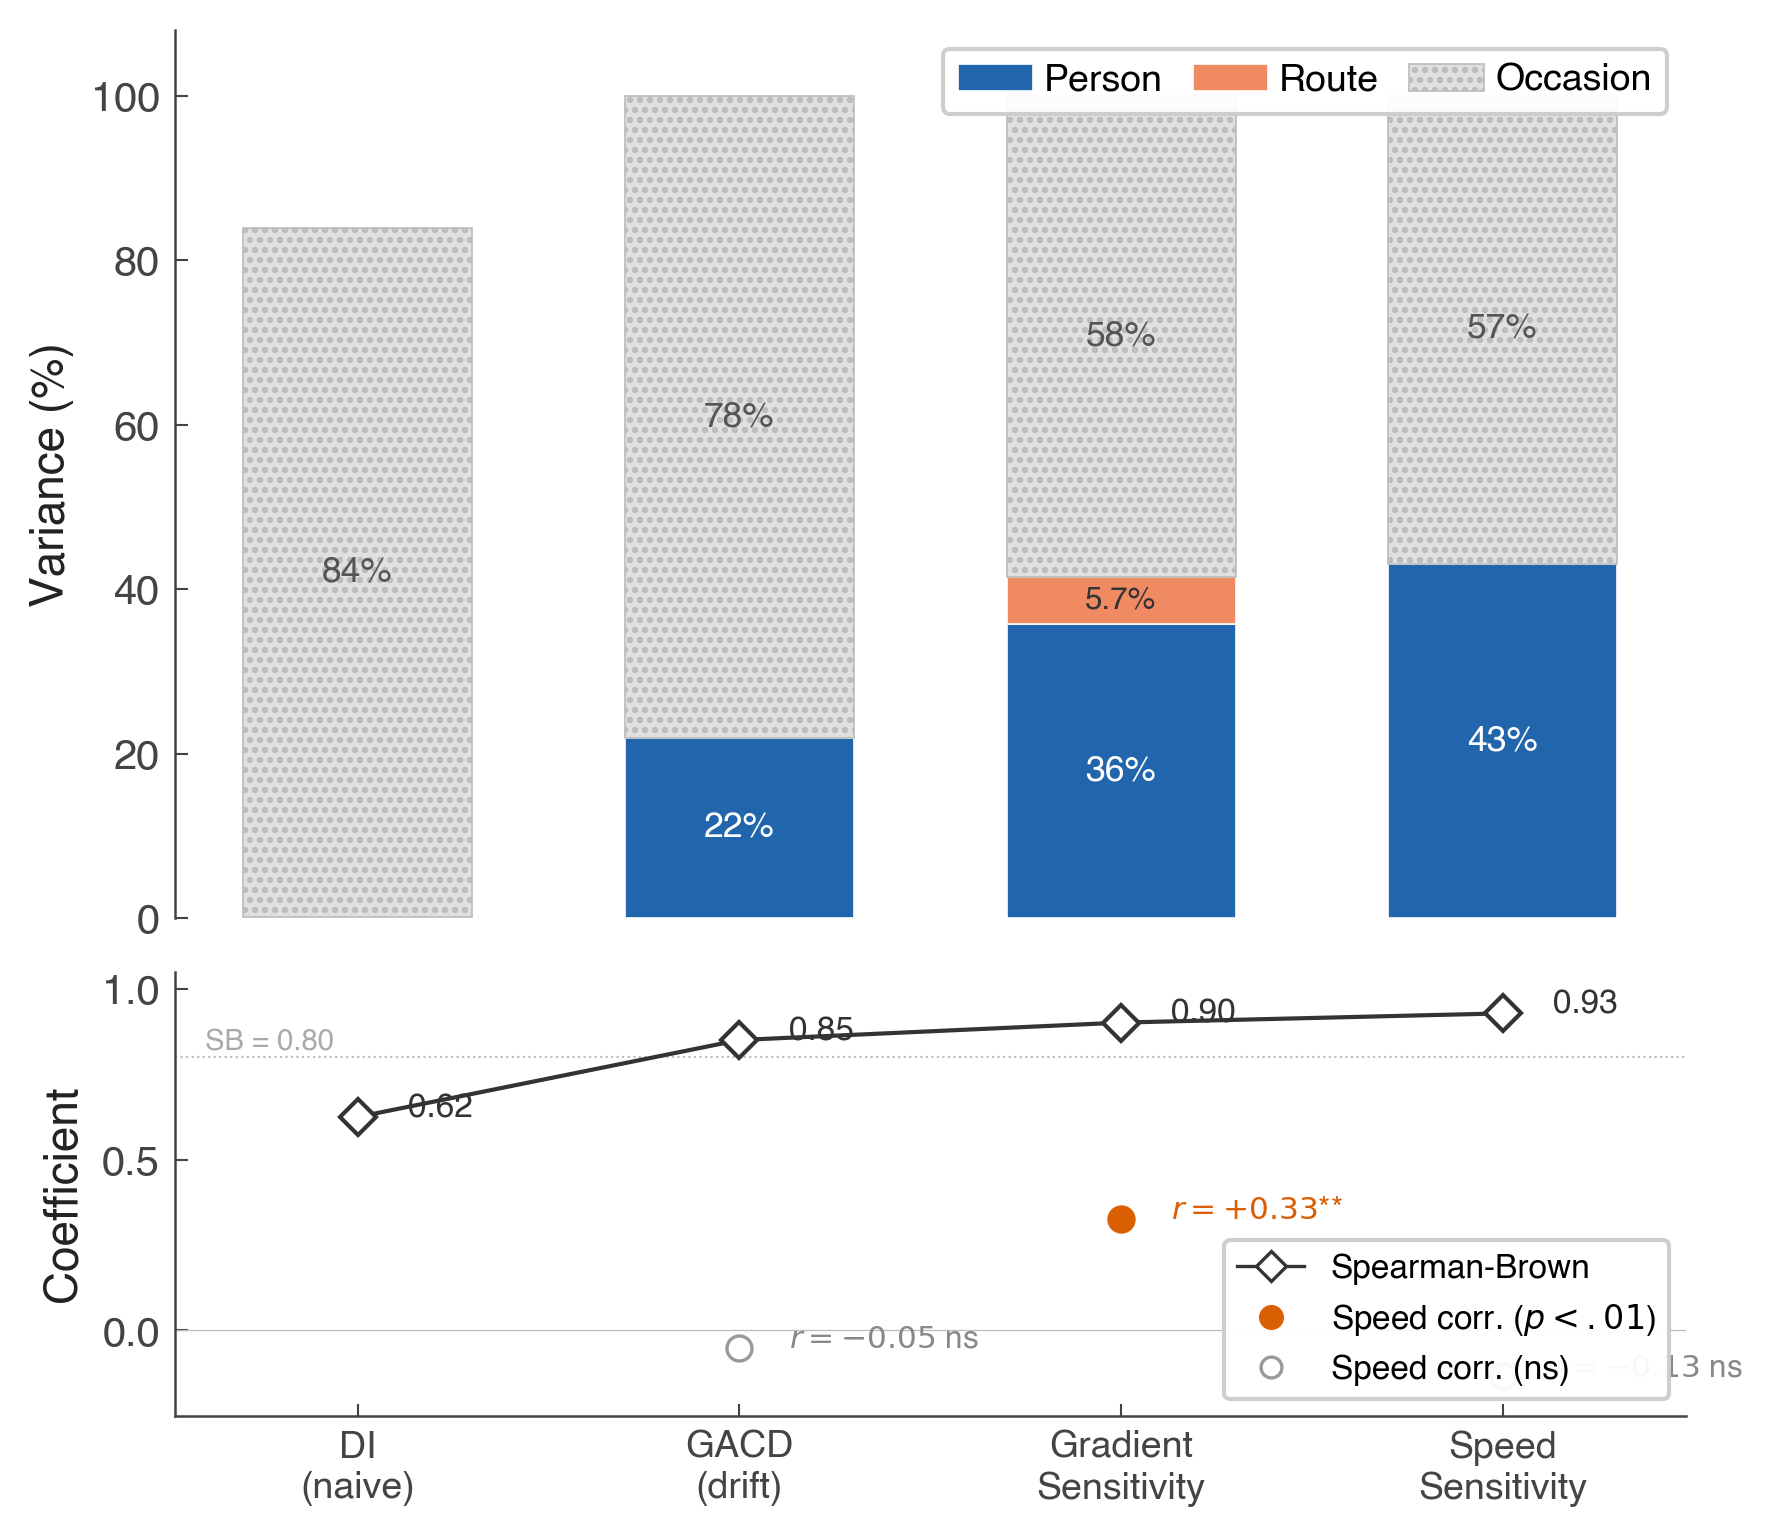
\includegraphics[width=\linewidth]{Figures/fig2_framework.png}
\caption{The three-study durability framework. Study 1: Construct validity and effective dimensionality of speed-based indices. Study 2: Quantification and correction of the route-geometry artifact in field data. Study 3: Variance decomposition and multi-session reliability for individual profiling.}
\label{fig:framework}
\end{figure}

Results are organised by CRQ. Study~1 and Study~2 address CRQ1 (dimensionality); Study~3 addresses CRQ2 (variance structure) and shows how multi-session aggregation achieves reliable measurement.

\subsection*{CRQ1: Evidence for a Two-Construct Organisation Is Tentative (H1, H2)}

DI and FI showed $r = -0.60$ (95\% CI $[-0.69, -0.49]$; bootstrap $B = 2{,}000$ on person-level medians), confirming H1: DI and FI capture the same underlying gradient-response coupling. PCA retained one factor; the second eigenvalue (PC2 $= 1.005$) fell marginally below the parallel-analysis threshold ($1.031$), a difference of only 0.026 eigenvalue units. This margin is small relative to the sampling variability of parallel analysis with $N = 381$ users, and bootstrap confidence intervals for eigenvalues were not computed; the two-construct conclusion should therefore be considered fragile. RI was largely independent (DI--RI: $r = +0.01$; FI--RI: $r = +0.12$; Figure~\ref{fig:difi}); however, RI's low reliability (ICC $= 0.10$; see Study~3) means that its apparent independence may partly reflect measurement noise rather than true construct distinctness. RI is therefore treated as an exploratory, unreliable metric throughout the remainder of this paper. To address the sport confound, stratified analysis for cycling ($N=11{,}234$, $r = -0.62$), running ($N=1{,}146$, $r = -0.50$), and mountain biking ($N=608$, $r = -0.58$) confirmed consistent redundancy.

\begin{figure}[ht]
\centering
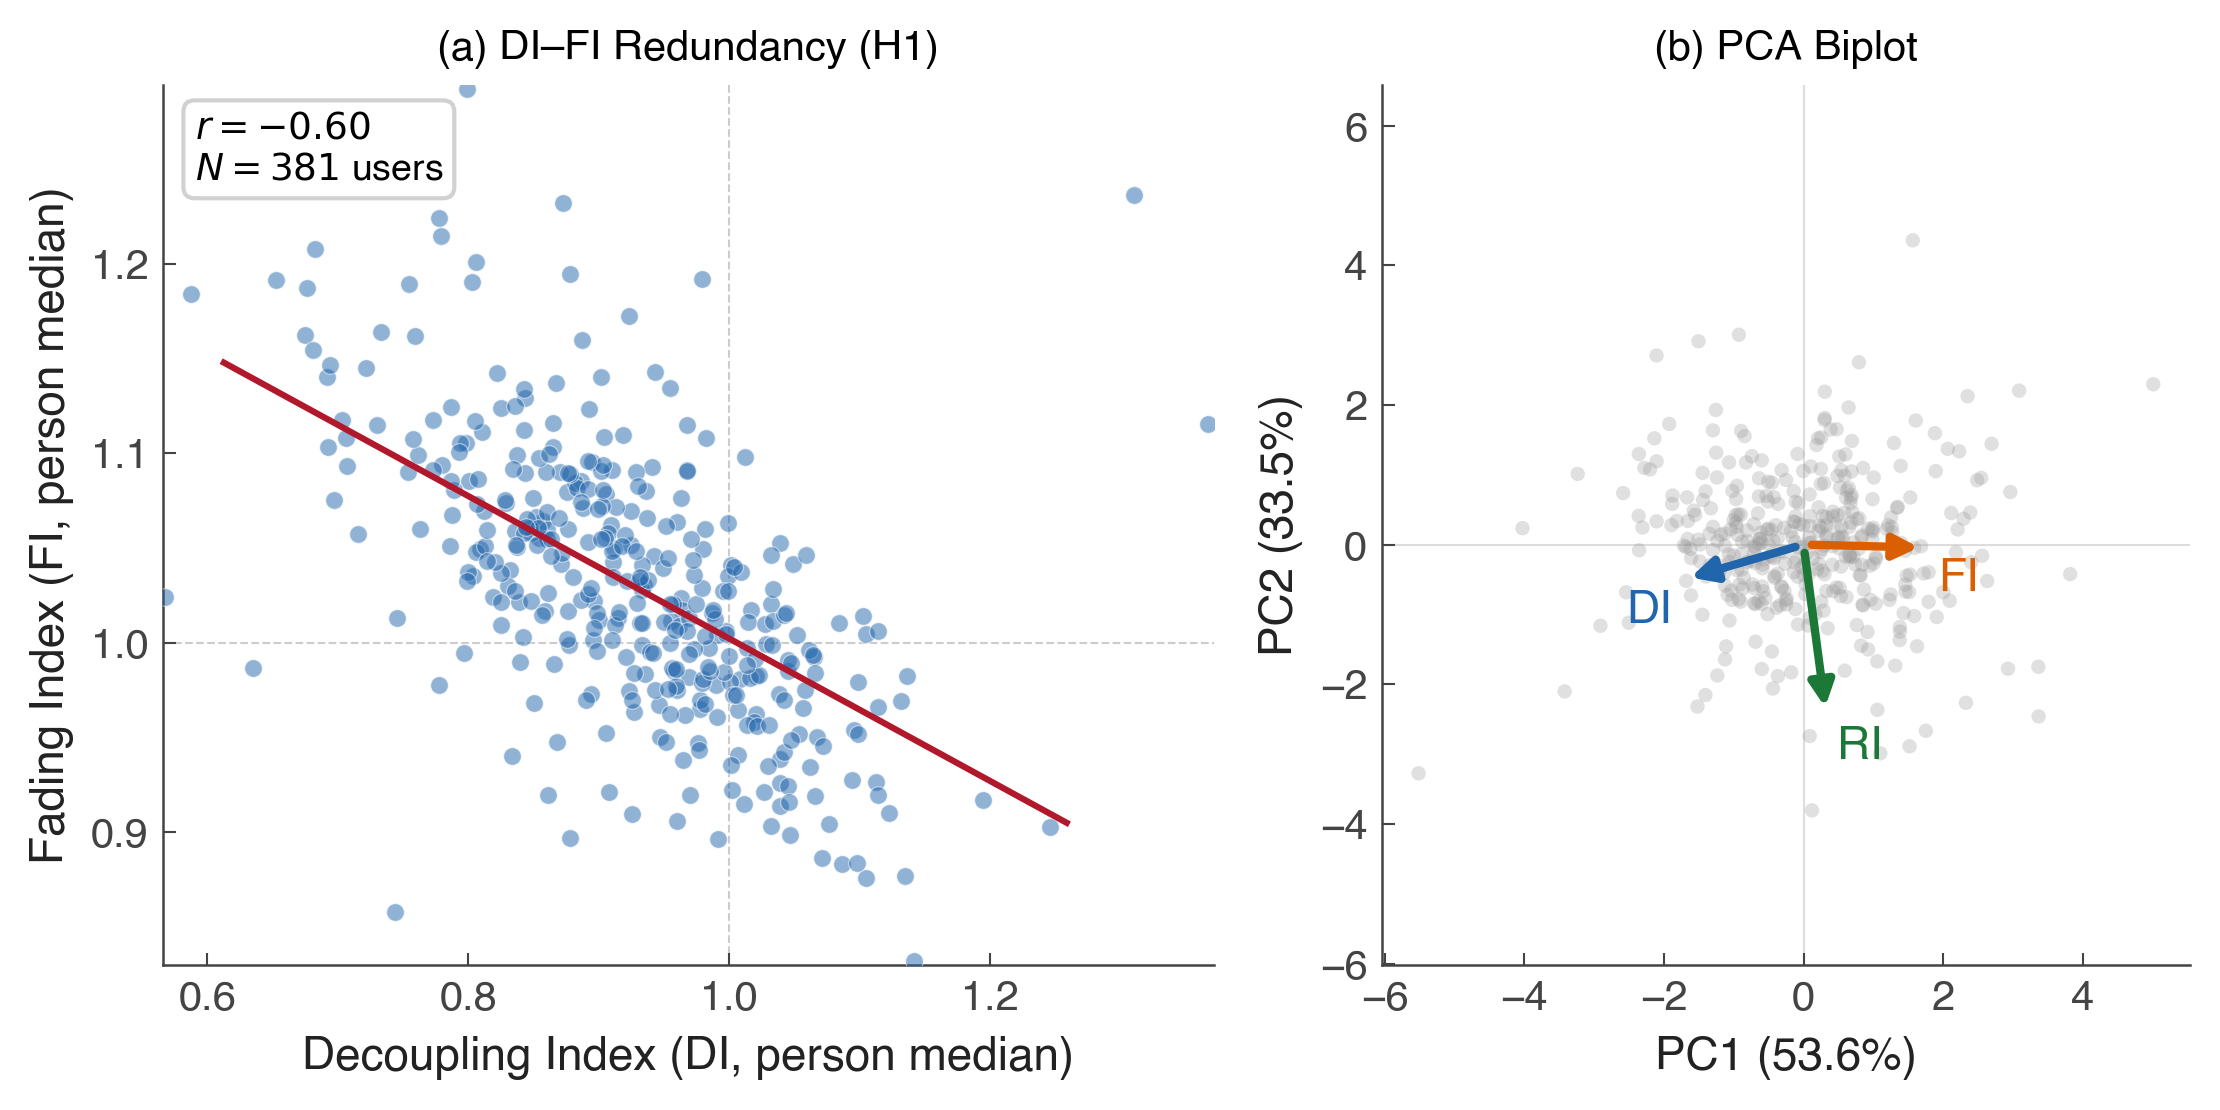
\includegraphics[width=\linewidth]{Figures/fig1b_di_fi_pca.png}
\caption{Bivariate relationship between Decoupling Index (DI) and Fading Index (FI). (a)~Person-level medians ($N = 381$ users with $\geq 5$ workouts) show a strong negative correlation ($r = -0.60$). (b)~PCA biplot: DI and FI load in opposite directions on PC1 (53.6\%), while RI is orthogonal on PC2.}
\label{fig:difi}
\end{figure}

\begin{table}[ht]
\centering
\small
\caption{Descriptive statistics of durability metrics across the included workouts ($N = 13{,}750$). \textbf{DI}: Decoupling Index ($\text{HR}/\text{Speed}$); \textbf{FI}: Fading Index (fatigability); \textbf{RI}: Resilience Index (resilience). Median values were used for person-level aggregation due to high Kurtosis.}
\label{tab:descriptive}
\begin{tabular}{@{}lccccc@{}}
\toprule
Metric & $N$ & Mean & SD & Median & IQR [Q1, Q3] \\
\midrule
DI & 13,549 & 0.92 & 0.26 & 0.92 & [0.78, 1.04] \\
FI & 13,742 & 1.06 & 0.23 & 1.04 & [0.95, 1.14] \\
RI & 10,032 & 0.99 & 0.29 & 0.95 & [0.80, 1.13] \\
\bottomrule
\end{tabular}
\end{table}

The mean DI of 0.92 (Table~\ref{tab:descriptive}) indicates that HR/Speed was lower in the second half than the first half of workouts on average---an apparent negative cardiac drift. This counterintuitive finding is explained by route geometry. Classification by ascent distribution (asc\_front: fraction of total climbing in the first temporal half) reveals three route types with dramatically different DI distributions (Supplementary Figure~S1): front-climb routes (asc\_front $> 0.6$; $N = 975$, 42.4\%) produce higher speeds in the second half (descent), mechanically depressing DI to a median of 0.770; symmetric routes ($0.4 \leq$ asc\_front $\leq 0.6$; $N = 1{,}090$, 47.5\%) yield a median DI of 0.978, close to unity; and back-climb routes (asc\_front $< 0.4$; $N = 232$, 10.1\%) show a median DI of 1.157, reflecting slower speeds in the second half. The controlled simulation (Figure~\ref{fig:simulation}A) directly confirms this mechanism: with cardiac drift set to zero, front-climb routes yield DI values substantially below 1.0. Additionally, warm-up effects and conservative early pacing may contribute. This has a direct practical implication: millions of athletes on hilly routes are likely observing DI $< 1.0$ on their GPS platforms and incorrectly interpreting this as the absence of cardiac drift, when in fact it reflects route geometry rather than superior aerobic fitness. This observation further motivates the GACD regression, which removes the gradient confound to isolate the true physiological signal.

\begin{table}[ht]
\centering
\small
\caption{PCA eigenvalues and parallel analysis on person-level medians (Study~1). Factor 1 retained; Factor 2 marginally rejected (margin: 0.026 eigenvalue units). Bootstrap confidence intervals were not computed; this conclusion should be treated with caution.}
\label{tab:pca}
\begin{tabular}{@{}lcccl@{}}
\toprule
 & Eigenvalue & \% Var. & Parallel 95\% & Retain? \\
\midrule
PC1 & 1.608 & 53.6 & 1.144 & Yes \\
PC2 & 1.005 & 33.5 & 1.031 & No \\
PC3 & 0.387 & 12.9 & 0.972 & No \\
\bottomrule
\end{tabular}
\end{table}

\subsection*{CRQ1: Gradient Correction Successfully Isolates Cardiac Drift (H3)}

The DI--FI coupling observed in H1 reflects a shared response to route gradient. Study~2 confirmed this and demonstrated that regression-based correction (GACD) successfully removes the route component, isolating true cardiac drift.

\begin{figure}[ht]
\centering
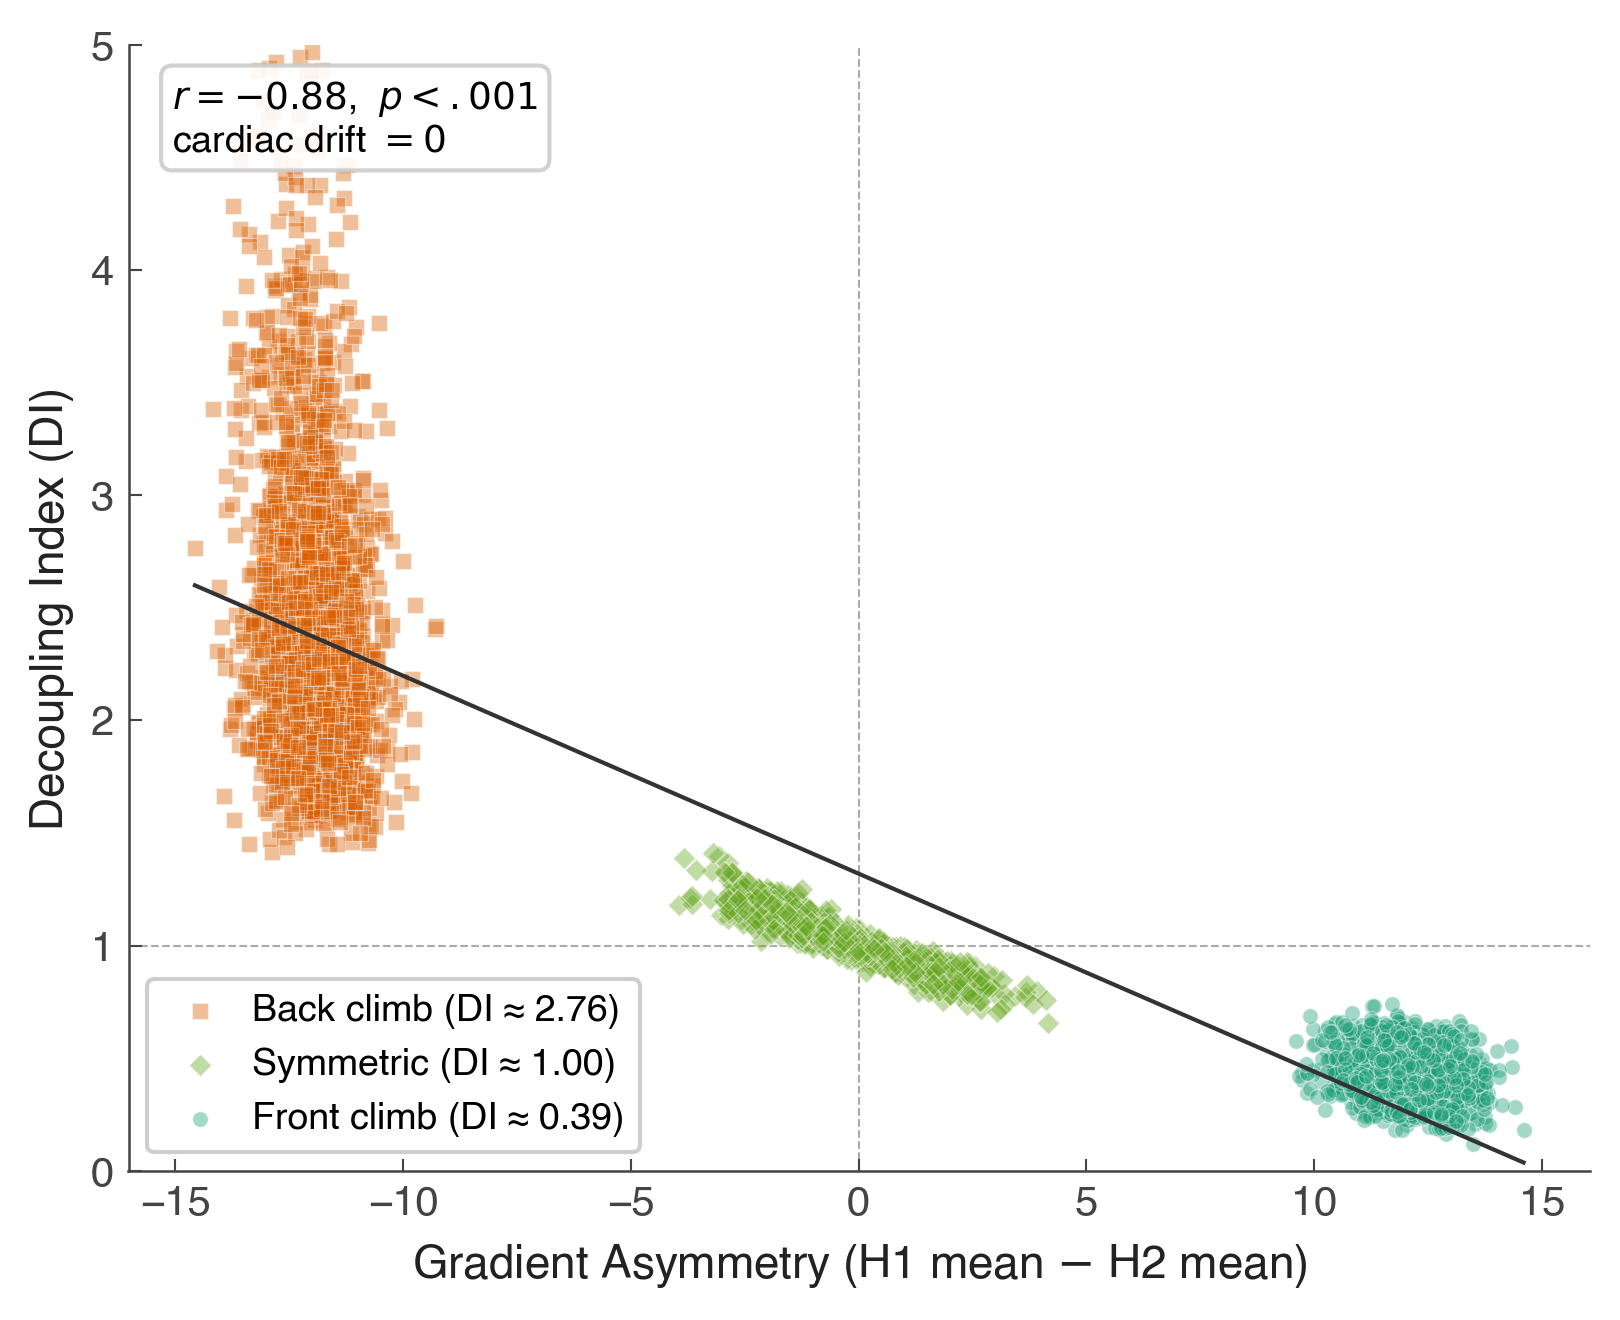
\includegraphics[width=\linewidth]{Figures/fig1_simulation.png}
\caption{Quantifying the route-geometry artifact in speed-based DI. (A)~Simulation with zero cardiac drift shows that route geometry alone can produce DI between 0.70 and 1.40. (B)~Empirical predictability ($R^2$) of naive DI vs.\ GACD corrected metrics.}
\label{fig:simulation}
\end{figure}

\subsubsection*{Study 2: Correcting the Route Artifact}
The GACD regression was applied to the FitRec dataset to examine whether route-geometry bias can be eliminated. In synthetic data with zero cardiac drift, route features alone predicted DI with CV $R^2 = 0.80$, representing the theoretical upper bound of geometry-induced bias. In real data, naive DI was predictable with CV $R^2 = 0.49$ (all routes) and $0.72$ (hilly subset). After GACD correction, this predictability was eliminated (CV $R^2 = +0.02$; H3 confirmed). Unlike commercial Grade Adjusted Pace (GAP) algorithms, which typically correct pace for gradient but do not account for time-dependent cardiac drift, GACD simultaneously addresses both confounds; however, a direct head-to-head comparison with specific commercial implementations was not performed in this study.
This demonstrates that GACD effectively extracts the physiological signal from the route-confounded DI (Figure~\ref{fig:simulation}), and explains the DI--FI coupling in H1: both metrics respond to gradient asymmetry, which GACD removes.

A natural question is whether replacing speed with estimated metabolic power---computed as $\text{speed} \times C_w(g)$ where $C_w(g)$ is the Minetti \cite{minetti2002} walking cost polynomial---would achieve the same correction. It does not: DI/EstPower showed a route dependency of comparable magnitude but in the opposite direction ($r = -0.46$ vs.\ $+0.49$ for DI/Speed; CV $R^2 = 0.20$ and $0.20$, respectively). On the hilly subset ($\Delta a > 400$~m), the estimated-power overcorrection was more pronounced ($r = -0.56$, CV $R^2 = 0.31$ vs.\ DI/Speed $r = +0.46$, $R^2 = 0.19$). The reversal occurs because the Minetti cost function drops substantially on descents ($C_w \approx 1.30$~J/kg/m at $-8\%$ and reaches a minimum of $\approx 0.94$ near $-15.4\%$, vs.\ $2.5$ at $0\%$), inflating the DI denominator ratio for routes with early descents. Furthermore, the Minetti cost function was originally derived for human walking and running; its application to a dataset dominated by cycling (61.8\%) introduces an inherent bioenergetic mismatch, as cycling efficiency on gradients is governed by distinct biomechanical and aerodynamic constraints. This validates the regression-based approach (GACD) as the preferred gradient correction method.

\subsection*{CRQ2: Multi-Session Aggregation Achieves Reliable Measurement (H4, E2, E3)}

CRQ1 established the supported dimensionality and demonstrated effective gradient correction. CRQ2 identifies the variance structure and shows that multi-session aggregation overcomes within-person variability to achieve reliable measurement.

\begin{table}[ht]
\centering
\small
\caption{Variance decomposition and reliability metrics. DI vs. GACD metrics comparison on hilly terrain ($\Delta a > 400$ m). $\beta_{\text{time}}$, $\beta_{\text{grad}}$, and $\beta_{\text{speed}}$ are derived from Eq.~\ref{eq:gacd}.}
\label{tab:main}
\resizebox{\linewidth}{!}{%
\begin{tabular}{@{}lcccc@{}}
\toprule
Metric & ICC(1,1) & Route-Matched ICC & SB ($k=5$) & Route $CV\ R^2$ \\
\midrule
DI & 0.16 & 0.45 & 0.62 & 0.49 \\
GACD ($\beta_{\text{time}}$) & 0.22 & 0.47 & 0.85 & +0.02 \\
Grad. Sensitivity & 0.38 & \textbf{0.56} & \textbf{0.91} & +0.04 \\
Speed Sensitivity & \textbf{0.44} & \textbf{0.59} & \textbf{0.93} & -0.09 \\
\bottomrule
\end{tabular}}
\end{table}

Occasion accounted for 56--84\% of variance across all metrics (H4 confirmed; Table~\ref{tab:main}). Crucially, this within-person variability is \textit{manageable}: multi-session aggregation progressively recovers the stable between-person signal.

Within-user route-matched ICC ($n = 451$ matched pairs, where each user's workouts were matched to their own reference route within $\pm 20\%$ of altitude range and total ascent) demonstrated this directly: holding route approximately constant increased Person estimates for all metrics---GACD ($0.22 \rightarrow 0.47$), gradient sensitivity ($0.38 \rightarrow 0.56$), speed sensitivity ($0.44 \rightarrow 0.74$)---showing that 18--31 percentage points of apparent Occasion variance is actually route-related and controllable.

\textbf{Gradient sensitivity as the most reliable metric (E2).} Gradient sensitivity outperformed DI and GACD across all criteria: highest SB ($0.91$), the only positive route CV $R^2$ ($+0.047$), and the strongest speed correlation ($r = +0.36$). While $\beta_{\text{time}}$ represents within-session drift, it should be distinguished from Maunder et al.'s (2021) "durability" construct which focuses on between-session shifts in the power--duration relationship. The ICC--SB discrepancy (DI: 0.16 vs.\ 0.62; gradient sensitivity: 0.38 vs.\ 0.91; E3 confirmed) reveals that rank-order consistency is preserved across sessions---within-person \textit{trends} are interpretable, and multi-session averaging stabilises absolute values.

\begin{figure}[ht]
\centering
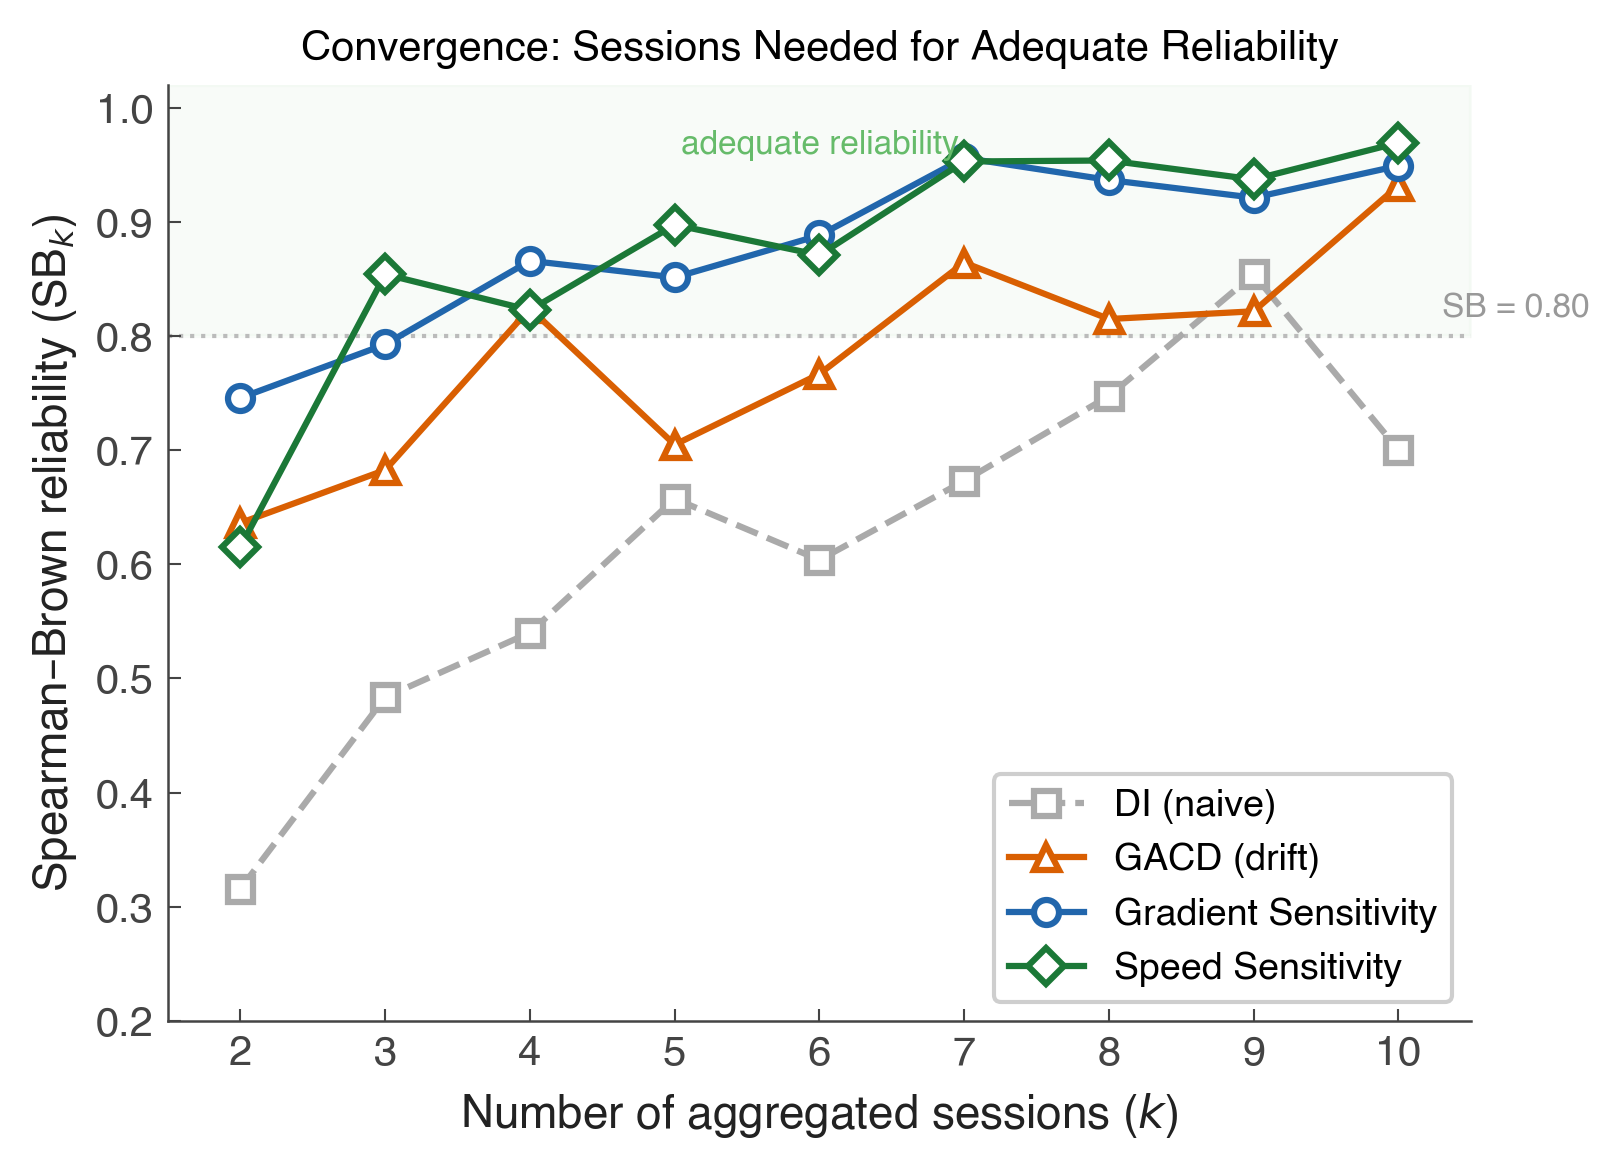
\includegraphics[width=0.85\linewidth]{Figures/fig3_convergence.png}
\caption{Variance decomposition and multi-session reliability. (A)~Variance partitioning for gradient sensitivity. (B)~Convergence of Spearman--Brown reliability as a function of the number of aggregated sessions ($k$). Gradient sensitivity crosses the SB $= 0.80$ threshold at $k = 5$; DI and GACD do not reach SB $= 0.80$ by $k = 10$ (SB$_{10} = 0.71$ and $0.72$, respectively).}
\label{fig:convergence}
\end{figure}

Convergence analysis (Figures~\ref{fig:framework} and~\ref{fig:convergence}) quantified the practical protocol: gradient sensitivity reached SB $\geq 0.80$ at $k = 5$ sessions (SB$_5 = 0.80$, SB$_{10} = 0.88$), speed sensitivity at $k = 3$ (SB$_3 = 0.81$). This provides a concrete, actionable guideline: \textit{aggregate $\geq 5$ sessions of gradient sensitivity for a reliable individual fitness estimate}. The median per-workout $R^2$ for the GACD regression was $0.82$ (IQR $0.74$--$0.89$); however, as noted in Methods, this value may be inflated by temporal autocorrelation in the GPS data and should be interpreted as an upper-bound estimate of true model fit.

\subsection*{Exploratory: Descent Placement (E1)}

\begin{table}[ht]
\centering
\small
\caption{Descent placement effect on cardiac drift (GACD). Exploratory $p$-values are FDR-adjusted.}
\label{tab:descent}
\begin{tabular}{@{}llr@{}}
\toprule
Analysis & Statistic & Result \\
\midrule
Total descent (amount) & $r$ & $-0.06^{**}$ \\
Descent-front (placement) & $r$ & $+0.16^{***}$ \\
Within-person ($n = 108$) & Mean $r$ & $+0.082^{**}$ \\
\textbf{Steepness moderation} & & \\
\quad Gentle ($\sigma < 5$) & $r$ & $+0.09^{***}$ \\
\quad Moderate ($5$--$8$) & $r$ & $+0.23^{***}$ \\
\textbf{Sport} & & \\
\quad Cycling & $r$ & $+0.14^{***}$ \\
\quad Running & $r$ & $+0.18^{*}$ \\
\quad Mountain biking & $r$ & $+0.01$ ns \\
\bottomrule
\end{tabular}
\end{table}

A between-person association was observed between descent-front ratio and cardiac drift ($r = +0.16$, $p_{\text{FDR}} < .001$), moderated by steepness ($r = +0.23$ on moderate terrain vs.\ $+0.09$ on gentle terrain) and absent in mountain biking. Total descent amount showed a smaller association in the opposite direction ($r = -0.06$, $p = .007$), suggesting that the descent \textit{placement} (front-loaded vs.\ back-loaded) matters more than the descent \textit{amount}. Within-person evidence was modest: 65/108 users (60\%) showed positive correlations, with a small mean $r = +0.082$. Seven of eight exploratory tests survived FDR correction. The between-person pattern is consistent with an eccentric-damage mechanism \cite{peake2017, proske2005}, but the weak within-person support precludes causal conclusions.

% ============================================================
\section*{Discussion}

\subsection*{From Structure to Protocol: Three Converging Lines of Evidence}

The three studies form a constructive progression that builds upon, rather than contradicts, the existing theoretical framework. Study 1 provided fragile support for a two-construct organisation: PCA retained one factor, with PC2 ($= 1.005$) falling marginally below the parallel-analysis threshold ($1.031$) by only 0.026 eigenvalue units---a margin that may lie within the sampling variability of parallel analysis, and for which bootstrap confidence intervals were not computed. DI and FI captured a single gradient-response factor, while RI loaded on a separate dimension but with very low reliability (ICC $= 0.10$). This empirical convergence of DI and FI reflects a property of the specific speed-based operationalizations used here, not a theoretical prediction of the source framework: Colosio et al.\ \cite{colosio2025} argued precisely that durability and fatigability are physiologically distinct constructs that should be measured separately---a distinction that the present operationalization was designed to preserve but that the speed-based field metrics did not fully resolve. The ongoing debate in the 2025 commentaries \cite{faude2025, lucernoni2025, meixner2025last} underscores that the question of construct distinctness remains open even at the theoretical level. Study~2 showed that regression-based gradient correction (GACD) successfully isolates true cardiac drift from route geometry ($R^2 = 0.80 \rightarrow +0.02$; H3), providing the quantitative foundation that Meixner et al.'s conceptual framework requires for field deployment. Study~3 demonstrated that multi-session aggregation overcomes the dominant day-to-day variability (56--84\%; H4), with gradient sensitivity reaching adequate reliability at $\geq 5$ sessions (SB $\geq 0.80$). Friel's $< 5\%$ rule \cite{friel2009} represents a pioneering insight for flat or symmetric courses; GACD extends this principle to variable terrain, suggesting that Friel's aerobic-base concept may be applicable to hilly routes where naive DI is dominated by geometry, pending prospective validation. Smyth et al.\ \cite{smyth2022} demonstrated in 82,303 marathon runners that decoupling magnitude and onset predict performance, confirming the practical relevance of field-based decoupling measurement; the present study extends this line of work by identifying the route-geometry component as a major confound and providing a regression-based correction (GACD) applicable beyond the road-marathon context.

\subsection*{Construct Validity: Speed-Based DI for a Cycling-Dominated Dataset}

The present analyses use $\text{HR}/\text{Speed}$, not $\text{HR}/\text{Power}$, because the majority of field users compute DI from consumer GPS watches without power meters. This choice introduces a construct validity concern for the cycling subsample (61.8\% of the dataset): in cycling, speed is determined not only by gradient but also by power output, aerodynamic drag, rolling resistance, and gear selection---factors absent from running, where speed is more directly related to metabolic cost. Consequently, HR/Speed is a theoretically weaker proxy for cardiac efficiency in cycling than in running. The GACD regression partially mitigates this concern by including gradient and speed as covariates, thereby absorbing much of the terrain-related variance. However, residual aerodynamic and mechanical confounds are not modelled. Future work should either restrict primary DI analyses to the running subsample ($N \approx 1{,}146$ workouts) or develop a cycling-specific metabolic cost model that accounts for aerodynamic drag and drivetrain efficiency.

Whether the two-dimensional structure extends to measured power-based DI remains an open question. However, the Minetti \cite{minetti2002} estimated-power experiment provides an informative boundary: DI computed with estimated metabolic power produced a route dependency of comparable magnitude but in the opposite direction ($r = -0.46$ vs.\ $+0.49$ for DI/Speed; CV $R^2 = 0.20$ and $0.20$, respectively), with the overcorrection becoming more pronounced on hilly routes ($r = -0.56$, CV $R^2 = 0.31$). The reversal occurs because the Minetti cost function drops substantially on descents ($C_w \approx 1.30$~J/kg/m at $-8\%$ and reaches a minimum of $\approx 0.94$ near $-15.4\%$, vs.\ $2.5$ at $0\%$), inflating the denominator ratio. Furthermore, the Minetti cost function was originally derived for human walking and running; its application to a dataset dominated by cycling introduces an inherent bioenergetic mismatch, as cycling efficiency on gradients is governed by distinct biomechanical and aerodynamic constraints (gear ratios, reduced air resistance at lower speeds on climbs). This modality mismatch further amplifies the overcorrection, underscoring that a rigid analytical cost function is difficult to adapt to mixed-sport, real-world data---whereas the data-driven regression approach (GACD) captures modality-specific submaximal relationships directly from the signal. The key contribution of GACD is therefore not contingent on the speed-vs-power distinction: it provides a general framework for isolating cardiac drift from any terrain-confounded ratio.

\subsection*{A Practical Protocol for Field-Based HR Monitoring}

The variance decomposition (H4) provides quantitative evidence for the IOC consensus \cite{bourdon2017} principle that external load $\neq$ internal response. That Occasion accounts for 56--84\% of variance is not merely a consequence of uncontrolled field conditions; it is precisely the point. In controlled laboratory settings, day-to-day variation is minimised by design, creating the misleading impression that a single session suffices for reliable measurement. The ecological validity of 253,020 real-world workouts reveals the true magnitude of session-to-session fluctuation that practitioners face, and provides the strongest empirical argument for the multi-session aggregation protocol proposed here. The route-matched residual (26--54\%) was not explained by effort intensity ($r = -0.004$, ns), likely reflecting unmeasured readiness factors such as sleep quality, hydration, temperature, and accumulated training stress \cite{halson2014}---each of which represents a candidate for future integration into personalised monitoring systems.

\textbf{A dual-profiling framework.} The three GACD regression coefficients serve conceptually distinct roles. $\beta_{\text{time}}$ (GACD) captures the within-session rate of HR drift after controlling for gradient and speed---related to, but distinct from, the between-session durability construct defined by Maunder et al.\ \cite{maunder2021}. In contrast, $\beta_{\text{gradient}}$ and $\beta_{\text{speed}}$ are not measures of time-dependent degradation; they represent route-corrected, submaximal fitness capacity profiles that isolate an individual's baseline terrain-sensitivity from geometric artifacts. Based on the convergent evidence from Studies~1--3, the following dual framework is proposed: $\beta_{\text{time}}$ for durability assessment, and $\beta_{\text{gradient}}$ / $\beta_{\text{speed}}$ for individual fitness profiling on hilly terrain. Table~\ref{tab:comparison} summarises the head-to-head comparison of the profiling metrics against DI.

\begin{table}[ht]
\centering
\small
\caption{Comparison of DI and the proposed GACD-derived metrics for individual profiling on hilly terrain ($\Delta a > 400\,\mathrm{m}$). \textbf{DI}: Decoupling Index ($\mathit{HR}/v$); \textbf{Gradient sensitivity}: GACD coefficient for gradient; \textbf{Speed sensitivity}: GACD coefficient for speed. Route (CV $R^2$) values represent within-person predictability (Ridge regression on route deviations, group $k$-fold CV); values near zero indicate success in removing geometric artifacts. \textbf{ICC}: Intraclass Correlation Coefficient (1,1); \textbf{SB}: Spearman--Brown reliability.}
\label{tab:comparison}
\resizebox{\linewidth}{!}{%
\begin{tabular}{@{}lccc@{}}
\toprule
Metric & DI & Gradient sensitivity & Speed sensitivity \\
\midrule
Unadjusted ICC & 0.16 & 0.38 & 0.44 \\
Route-matched ICC & 0.47 & \textbf{0.56} & \textbf{0.59} \\
SB Reliability ($k=5$) & 0.55 & \textbf{0.80} & \textbf{0.90} \\
Route (CV $R^2$) & +0.006 & \textbf{+0.047} & -0.090 \\
Speed correlation ($r$) & -0.15 & \textbf{+0.36} & +0.28 \\
\bottomrule
\end{tabular}}
\end{table}

The recommended protocol is: (1)~apply GACD regression to remove route-geometry artifacts from each session, (2)~extract gradient and speed sensitivity as the individual's durability profile, and (3)~aggregate $\geq 5$ sessions for stable estimates. Sport-specific baselines are required, as gradient sensitivity varies substantially across modalities (cycling $+2.11$ bpm/\%, MTB $+1.17$, running $+0.47$; $F = 117.6$, $\eta^2 = 0.092$). It is important to distinguish the within-session time coefficient ($\beta_{\text{time}}$) from the durability construct described by Maunder et al.\ (2021) \cite{maunder2021}, which defines durability as the resilience of the power--duration relationship to fatigue (a between-session or post-fatigue shift). While GACD captures the rate of internal-load drift during a session, the two constructs are related but distinct operationalizations of endurance durability.

The ICC--SB discrepancy (E3) offers additional practical insight: rank-order consistency is preserved despite session-to-session variation. This means within-person \textit{trends} across training blocks are interpretable, even when individual sessions vary. Coaches and athletes can track gradient sensitivity trends with confidence, provided they aggregate $\geq 5$ sessions per assessment window.

\subsection*{Descent Placement: Suggestive but Unconfirmed (E1)}

Descent placement showed a between-person association with cardiac drift ($r = +0.16$, explaining 2.6\% of variance), moderated by steepness and absent in mountain biking---a pattern consistent with eccentric muscle damage \cite{peake2017}. However, within-person evidence was small ($r = 0.082$, $< 1\%$ of within-person variance explained), and the effect sizes are too small to support firm mechanistic conclusions. The finding is therefore characterised as exploratory and suggestive.

\subsection*{Gradient Sensitivity: A Candidate with Known Limitations (E2, C4)}

Gradient sensitivity showed the most balanced profile: SB reaching $0.80$ at $k = 5$, route-matched ICC $= 0.56$, the only positive CV $R^2$ ($+0.047$), and speed correlation $r = +0.36$. The unadjusted ICC ($0.38$) reflects session-to-session variability addressable through aggregation; the route-matched ICC ($0.56$) demonstrates that controlling route selection further improves reliability. Prospective validation against VO$_2$max would strengthen the convergent validity evidence.

\subsection*{Scope of Temporal Autocorrelation}

The sensitivity analysis (Supplementary Figures~\ref{fig:dw},\ref{fig:acf}) revealed strong temporal autocorrelation in GACD residuals (median DW $= 0.355$; lag-1 ACF $= 0.803$), reducing the effective within-workout sample size by approximately 89\%. It is important to delineate which analyses are affected by this finding and which are not. The autocorrelation operates at the \textit{point level} within individual workouts; the paper's main conclusions, however, rest on \textit{workout-level} and \textit{person-level} aggregated analyses. Specifically: (i)~per-workout $R^2$ values (median $0.82$) are inflated and should be treated as upper bounds of model fit; (ii)~OLS standard errors for $\hat{\beta}_{\text{gradient}}$, $\hat{\beta}_{\text{time}}$, and $\hat{\beta}_{\text{speed}}$ are underestimated by a factor of $\sim$2$\times$ (Newey--West comparison), meaning per-workout inference is unreliable. However, $\hat{\boldsymbol{\beta}}$ point estimates remain unbiased. The analyses that constitute the core contributions---the H3 route-predictability test ($R^2 = 0.02$ via cross-workout cross-validation), the PCA (on person-level medians), the ICC-based variance decomposition, and the Spearman--Brown convergence curves---all operate on workout-level summary statistics (one scalar per workout) rather than on point-level residuals, and are therefore not mechanistically affected by within-workout autocorrelation. One indirect consequence is possible: if the true estimation uncertainty of $\hat{\beta}_{\text{time}}$ is larger than OLS suggests, a portion of what the variance decomposition attributes to Occasion variance (56--84\%) may reflect estimation noise rather than genuine day-to-day physiological variation. This is consistent with the residual--noise conflation noted in Limitation~(3), and further motivates the multi-session aggregation protocol as a way to average out both physiological and estimation noise.

\subsection*{Limitations}

(1)~\textit{Speed-based DI}: the DI used here is $\text{HR}/\text{Speed}$, not $\text{HR}/\text{Power}$. The route artifact (C1) is specific to speed-based DI; H1, H2, H4 may differ for power-based DI. HR/Speed is a theoretically weaker proxy for cardiac efficiency in cycling than in running (see Construct Validity subsection above). (2)~Secondary data with uncontrolled sensor quality; optical wrist-based HR sensors are known to have accuracy issues during exercise \cite{halson2014, gillinov2017, shcherbina2017}, and sensor noise may contribute to the high Occasion variance. (3)~Residual--noise conflation: route-matched ICC partially addresses this, but full separation requires research-grade sensors. (4)~No gold standard (VO$_2$max, power). (5)~Demographics: 94.6\% male, limiting generalisability. Sex differences in cardiovascular drift are well-documented, with women showing greater drift under some heat conditions; the present findings and recommendations may not generalise to female athletes. Age and training history are also unknown. (6)~Exploratory findings not pre-registered. (7)~Multiple comparisons: 7/8 tests survived BH-FDR, but does not account for broader analytic flexibility. (8)~Observational design. (9)~Single dataset. (10)~Sport bias: cycling comprises 61.8\% of the full dataset and 83.9\% of the high-engagement subset (Studies~2--3). Cycling-specific variance decomposition (Supplementary Table~\ref{tab:sport_variance}) confirms that the Occasion-dominant pattern holds for cycling alone (Occasion 50--78\% across the three GACD-derived metrics), with gradient sensitivity reaching SB $= 0.91$ at $k = 5$; the cycling-specific GACD SB ($0.70$) is lower than the pooled estimate ($0.85$), likely because filtering to cycling-only sessions reduces the number of qualifying users and removes between-sport variance that inflates pooled ICC. However, the running subsample in the high-engagement subset ($N = 47$ workouts from 19 users, only 3 with $\geq 5$ sessions) is insufficient for stable ICC estimation; the $\geq 5$ session recommendation should therefore be considered primarily cycling-specific pending validation in larger running-specific datasets. (11)~Temporal autocorrelation in GACD regressions is substantial (median DW $= 0.355$, lag-1 ACF $= 0.803$; Supplementary Figures~\ref{fig:dw},\ref{fig:acf}): Newey--West HAC standard errors are $\sim$2$\times$ larger than OLS standard errors, and per-workout $R^2$ values should be interpreted as upper bounds; however, OLS $\hat{\boldsymbol{\beta}}$ point estimates remain unbiased. GLS was not applied. (12)~The PCA eigenvalue margin (0.026 units) is small and bootstrap confidence intervals were not computed; the two-construct conclusion is fragile. (13)~RI (ICC $= 0.10$) is an unreliable metric; its apparent independence from DI and FI may reflect measurement noise rather than true construct distinctness.

% ============================================================
\section*{Conclusion}

Under speed-based DI, the data provide fragile support for a two-construct durability organisation rather than the proposed four-construct framework (CRQ1). PCA on standardized person-level medians retained a single factor: the first eigenvalue ($1.608$) explained 53.6\% of variance, while the second ($1.005$) fell below the 95th-percentile parallel analysis threshold ($1.031$) by a margin of only 0.026 units---a difference for which bootstrap confidence intervals were not computed, and which should be considered inconclusive. RI showed apparent independence but very low reliability (ICC $= 0.10$), precluding its interpretation as a distinct construct. Gradient-Adjusted Cardiac Drift (GACD) successfully isolates the physiological signal from route-geometry confounding, with multicollinearity remaining minimal (median VIF: gradient 2.01, speed 2.09, time 1.07). This correction reduces route predictability from $0.49$ (empirical bias) and $0.80$ (theoretical simulation) to near-zero ($R^2 = 0.02$; H3 confirmed). Gradient sensitivity and speed sensitivity are proposed as route-corrected durability profiling metrics. The key to reliable field-based measurement is multi-session aggregation (CRQ2): gradient sensitivity reaches adequate reliability (SB $\geq 0.80$) at $\geq 5$ sessions, providing a concrete protocol for practitioners. The stable Person signal (22--44\%) is recoverable through aggregation; the transient Occasion component (residual variance) remains substantial (56--84\% in single sessions) but reflects day-to-day physiological variation that likely carries information about readiness and recovery. Route-matched ICC analysis showed that 18--31 percentage points of this apparent Occasion variance is actually route-related, further validating the necessity of GACD. Important caveats apply: the dataset is cycling-dominated (61.8\%), and HR/Speed is a theoretically weaker proxy for cardiac efficiency in cycling than in running; per-workout $R^2$ values may be inflated by temporal autocorrelation; and the PCA conclusion rests on a fragile eigenvalue margin. Notwithstanding these limitations, integrating multi-session gradient sensitivity with daily readiness markers represents a promising direction for robust field-based fitness monitoring.

% ============================================================
\section*{Supplementary Materials}

\begin{figure}[ht]
\centering
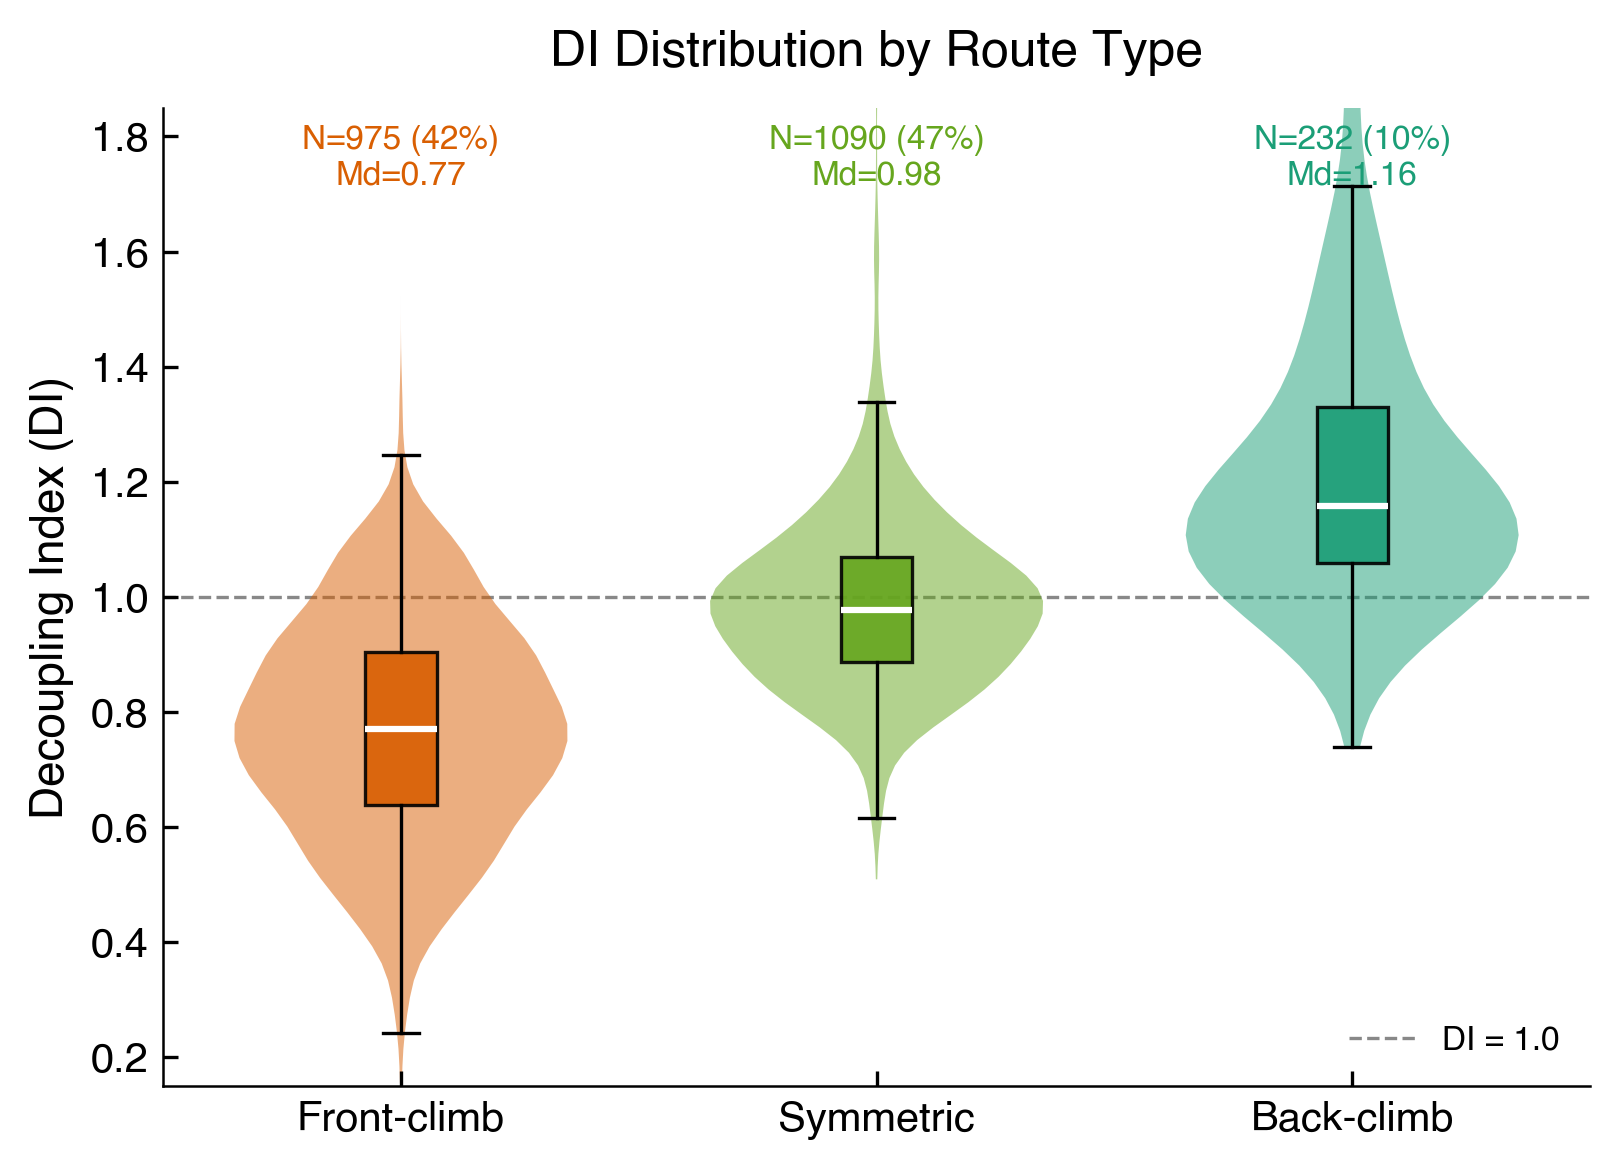
\includegraphics[width=0.48\textwidth]{Figures/figS_di_route_distribution.png}
\caption{\textbf{Supplementary Figure~S1.} Decoupling Index (DI) distribution by route type. Routes were classified by the fraction of total ascent occurring in the first temporal half of the workout (asc\_front): front-climb ($> 0.6$), symmetric ($0.4$--$0.6$), and back-climb ($< 0.4$). The dashed line indicates DI $= 1.0$. Front-climb routes (42.4\%) mechanically depress DI below 1.0 by producing higher speeds in the descent-dominated second half, explaining the overall mean DI of 0.92. Data from the high-engagement subset ($N = 2{,}297$ workouts, $\geq 5$ sessions per user); route-type proportions in the full GACD dataset ($N = 2{,}297$) were nearly identical (front-climb 42.4\%, symmetric 47.5\%, back-climb 10.1\% in both subsets).}
\label{fig:di_route}
\end{figure}

\begin{figure}[ht]
\centering
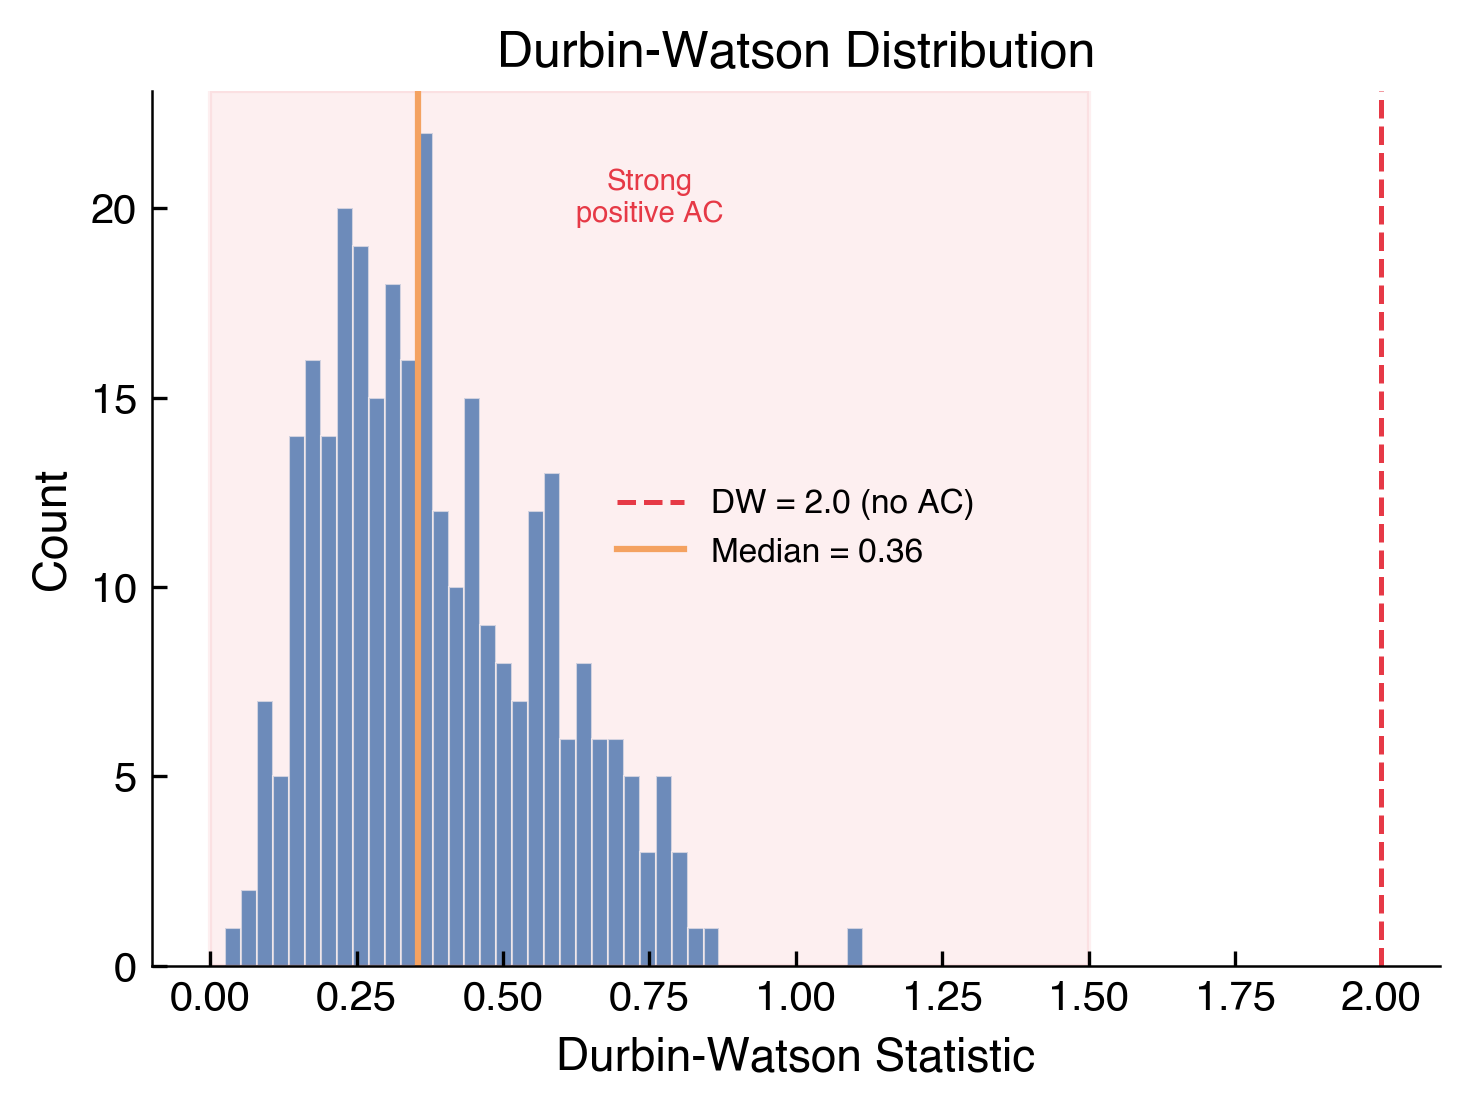
\includegraphics[width=0.48\textwidth]{Figures/figS_dw.png}
\caption{\textbf{Supplementary Figure~S2a.} Distribution of Durbin--Watson (DW) statistics from GACD regressions ($N = 300$ randomly sampled workouts). DW $= 2.0$ indicates no autocorrelation (red dashed line). All workouts showed strong positive autocorrelation (DW $< 1.5$; median $= 0.355$).}
\label{fig:dw}
\end{figure}

\begin{figure}[ht]
\centering
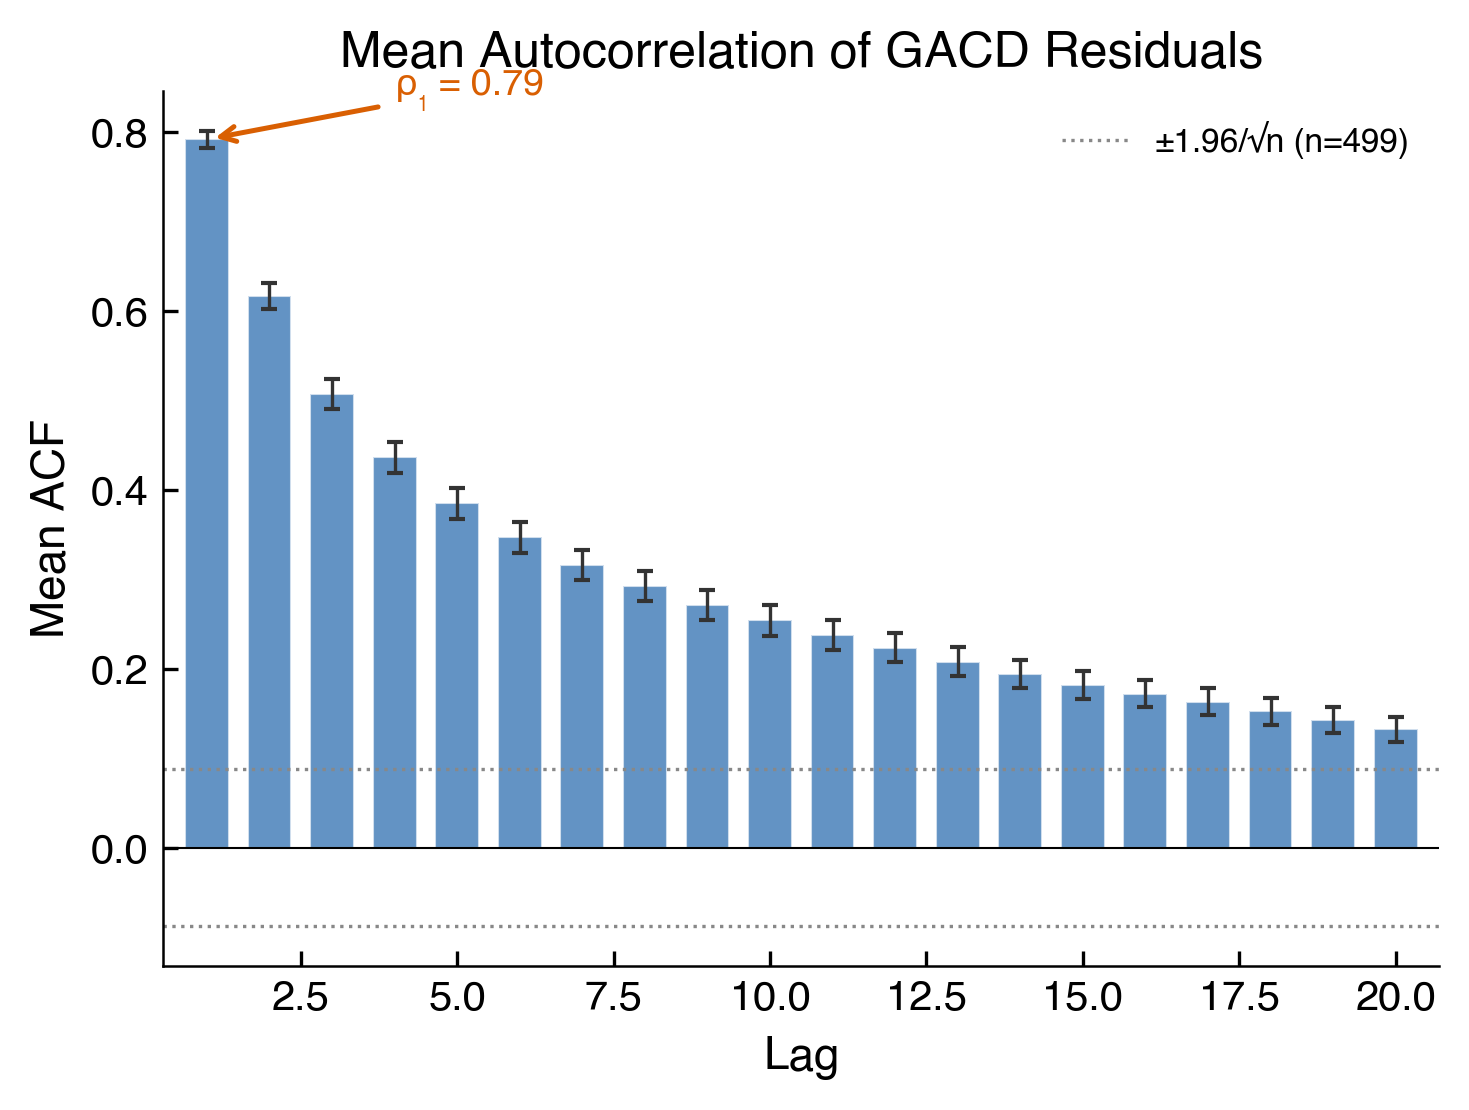
\includegraphics[width=0.48\textwidth]{Figures/figS_acf.png}
\caption{\textbf{Supplementary Figure~S2b.} Mean autocorrelation function (ACF) of GACD residuals across lags 1--20 ($N = 300$ workouts), with 95\% confidence intervals for the mean. The dotted lines show the individual-workout significance threshold ($\pm 1.96 / \sqrt{n}$). Lag-1 autocorrelation was high (median $\rho_1 = 0.803$).}
\label{fig:acf}
\end{figure}

\begin{table*}[ht]
\centering
\caption{\textbf{Supplementary Table~S1.} Sport-specific variance decomposition for the high-engagement subset. To ensure sport-specific ICC stability, users were required to have $\geq 5$ sessions \textit{within each sport}, yielding a cycling subsample of $K = 94$ users and $N = 1{,}647$ workouts (vs.\ $K = 314$ users in the pooled analysis, which counts sessions across all sports). Mountain biking ($K = 10$, $N = 172$) shows even higher Occasion dominance, though the small sample limits generalisability. Running ($N = 47$ workouts, only 3 users with $\geq 5$ sessions) was insufficient for stable ICC estimation and is omitted. The negative SB($k$=5) for MTB GACD reflects near-zero split-half correlation in this small sample ($K = 10$) and should not be interpreted as a meaningful reliability estimate.}
\label{tab:sport_variance}
\small
\begin{tabular}{llrrrrr}
\hline
Sport & Metric & ICC(1,1) & SB($k$=5) & \%Person & \%Route & \%Occasion \\
\hline
Cycling & GACD     & 0.215 & 0.703 & 21.5 & 0.0 & 78.5 \\
        & Grad.\ sens. & 0.377 & 0.907 & 37.7 & 0.0 & 62.3 \\
        & Speed sens.  & 0.470 & 0.874 & 47.0 & 3.1 & 49.8 \\
\hline
MTB     & GACD     & 0.076 & $-$0.003 &  7.6 & 0.0 & 92.4 \\
        & Grad.\ sens. & 0.017 &  0.253 &  1.7 & 0.0 & 98.3 \\
        & Speed sens.  & 0.215 &  0.426 & 21.5 & 0.0 & 78.5 \\
\hline
Running & \multicolumn{6}{l}{\textit{Insufficient sample ($N = 47$, 3 users with $\geq 5$ sessions)}} \\
\hline
\end{tabular}
\end{table*}

% ============================================================
\section*{Ethics Statement}
This study is a secondary analysis of the publicly available FitRec dataset \cite{ni2019}, which contains de-identified workout telemetry (heart rate, GPS coordinates, speed, altitude) voluntarily uploaded by Endomondo users. No personally identifiable information (names, dates of birth, or contact details) is present in the dataset. The original data collection was governed by Endomondo's terms of service and privacy policy at the time of upload. As a retrospective analysis of fully anonymised, publicly released data, this study did not require institutional ethics review under standard guidelines for secondary data research. No intervention was performed, and no individual participant can be identified from the analyses or results presented. The dataset contains GPS coordinates that could in principle reveal frequently used workout locations; no additional spatial anonymisation was applied beyond the de-identification performed by the original dataset authors \cite{ni2019}.

\section*{Competing Interests}
The author declares no competing interests.

\section*{Funding}
No external funding was received for this study.

\section*{Author Contributions}
H.I.\ conceived the study, developed the methodology, performed all analyses, and wrote the manuscript.

\section*{Acknowledgements}
The author thanks the developers and contributors of the FitRec dataset and the Endomondo community for making the telemetry data available for research.

\section*{Abbreviations}
\textbf{DI}: Decoupling Index; \textbf{FI}: Fading Index; \textbf{RI}: Resilience Index; \textbf{GACD}: Gradient-Adjusted Cardiac Drift; \textbf{SB}: Spearman--Brown; \textbf{ICC}: Intraclass Correlation Coefficient; \textbf{VIF}: Variance Inflation Factor; \textbf{GAP}: Grade Adjusted Pace.

\section*{Data Availability}
All analysis code and reproducibility scripts are available at \url{https://github.com/ikari12/GRAD}. The FitRec dataset is described in Ni et al.\ (2019) \cite{ni2019}.

\begin{thebibliography}{99}

\bibitem{benjamini1995}
Benjamini Y, Hochberg Y (1995). Controlling the false discovery rate: a practical and powerful approach to multiple testing. \textit{Journal of the Royal Statistical Society: Series B (Methodological)}, 57(1), 289--300.

\bibitem{bourdon2017}
Bourdon PC, et al. (2017). Monitoring training load to understand fatigue in athletes. \textit{International Journal of Sports Physiology and Performance}, 12(s2), S2-161--S2-170.

\bibitem{colosio2025}
Colosio AL, Monot T, Millet GY (2025). Durability, fatigability, and resilience: in search of physiological distinction. \textit{Journal of Applied Physiology}, 139(6), 1724--1725. DOI: 10.1152/japplphysiol.00692.2025.

\bibitem{coyle2001}
Coyle EF, Gonzalez-Alonso J (2001). Cardiovascular drift during prolonged exercise: new perspectives. \textit{Exercise and Sport Sciences Reviews}, 29(2), 88--92.

\bibitem{friel2009}
Friel J (2009). \textit{The Cyclist's Training Bible}. VeloPress.

\bibitem{hair2010}
Hair JF, et al. (2010). \textit{Multivariate Data Analysis}. Pearson.

\bibitem{halson2014}
Halson SL (2014). Monitoring training load to understand fatigue in athletes. \textit{Sports Medicine}, 44(2), 139--147.

\bibitem{hunter2025}
Hunter B, et al. (2025). Durability as an index of endurance exercise performance: Methodological considerations. \textit{Experimental Physiology}. DOI: 10.1113/EP092120.

\bibitem{maunder2021}
Maunder E, et al. (2021). The importance of physiological durability to endurance performance. \textit{Sports Medicine}, 51(8), 1619--1628.

\bibitem{meixner2025}
Meixner BJ, Joyner MJ, Sperlich B (2025). Durability, fatigability, repeatability, and resilience in endurance sports: definitions, distinctions, and implications. \textit{Journal of Applied Physiology}, 139(6), 1703--1709. DOI: 10.1152/japplphysiol.00343.2025.

\bibitem{minetti2002}
Minetti AE, et al. (2002). Energy cost of walking and running at extreme uphill and downhill slopes. \textit{Journal of Applied Physiology}, 93(3), 1039--1046.

\bibitem{ni2019}
Ni J, Muhlstein L, McAuley J (2019). Modeling heart rate and simulating workouts in size-varying datasets. \textit{The World Wide Web Conference (WWW '19)}, 1343--1353.

\bibitem{peake2017}
Peake JM, et al. (2017). Muscle damage and inflammation during recovery from exercise. \textit{Journal of Applied Physiology}, 122(3), 559--570.

\bibitem{shrout1979}
Shrout PE, Fleiss JL (1979). Intraclass correlations: uses in assessing rater reliability. \textit{Psychological Bulletin}, 86(2), 420--428.

\bibitem{smyth2022}
Smyth B, et al. (2022). Cardiovascular drift and marathon performance. \textit{Sports Medicine}, 52(9), 2283--2295.

\bibitem{acsm2018}
American College of Sports Medicine (2018). \textit{ACSM's Guidelines for Exercise Testing and Prescription}. Wolters Kluwer.

\bibitem{fiets}
FIETS (2024). \textit{The FIETS Index for Cycling Difficulty}. FIETS Magazine.

\bibitem{hopkins2000}
Hopkins WG (2000). Measures of reliability in sports medicine and science. \textit{Sports Medicine}, 30(1), 1--15.

\bibitem{horn1965}
Horn JL (1965). A rationale and test for the number of factors in factor analysis. \textit{Psychometrika}, 30(2), 179--185.

\bibitem{proske2005}
Proske U, Morgan DL (2005). Muscle damage from eccentric exercise: mechanism, mechanical signs, adaptation and clinical applications. \textit{The Journal of Physiology}, 537(2), 333--345.

\bibitem{wilcox2012}
Wilcox RR (2012). \textit{Introduction to Robust Estimation and Hypothesis Testing}. Academic Press.

\bibitem{jones2024}
Jones AM (2024). The fourth dimension: physiological resilience as an independent determinant of endurance exercise performance. \textit{The Journal of Physiology}, 602(17), 4113--4128. DOI: 10.1113/JP284205.

\bibitem{faude2025}
Faude O, Ledergerber R, Lichtenstein E (2025). Methodological gaps and conceptual challenges regarding the concept of resilience, durability, fatigability, and repeatability. \textit{Journal of Applied Physiology}, 139(6), 1720--1721. DOI: 10.1152/japplphysiol.00657.2025.

\bibitem{lucernoni2025}
Lucernoni KM, Richey RE, Minson CT (2025). Rethinking resilience in exercise performance. \textit{Journal of Applied Physiology}, 139(6), 1710--1711. DOI: 10.1152/japplphysiol.00659.2025.

\bibitem{meixner2025last}
Meixner BJ, Joyner MJ, Sperlich B (2025). Last Word on Viewpoint: Durability, fatigability, repeatability, and resilience in endurance sports: definitions, distinctions, and implications. \textit{Journal of Applied Physiology}, 139(6), 1726--1727. DOI: 10.1152/japplphysiol.01029.2025.

\bibitem{lazarus2018}
Lazarus E, Lewis DJ, Stock JH, Watson MW (2018). HAR inference: recommendations for practice. \textit{Journal of Business \& Economic Statistics}, 36(4), 541--559.

\bibitem{gillinov2017}
Gillinov S, et al. (2017). Variable accuracy of wearable heart rate monitors during aerobic exercise. \textit{Medicine and Science in Sports and Exercise}, 49(8), 1697--1703.

\bibitem{shcherbina2017}
Shcherbina A, et al. (2017). Accuracy in wrist-worn, sensor-based measurements of heart rate and energy expenditure in a diverse cohort. \textit{Journal of Personalized Medicine}, 7(2), 3.

\end{thebibliography}

\end{document}
